\label{chapter:using_machines}
\section{Checking whether a given bug is actually real}
\label{sect:using:check_realness}

Previous sections have described how to generate {\StateMachines}
which represent a given fragment of the program and how to simplify
them down to remove most of the redundant information.  This section
gives a mechanism for using those {\StateMachines} to check whether
running two fragments of the program in parallel might conceivably
lead to a crash and, if so, under what circumstances it might do so.

The core of the approach is to take a pair of {\StateMachines}, one
representing the read thread and the other representing the write
thread, and convert them into a verification condition using symbolic
execution\smh{Think you need to be clearer about terminology... e.g
  the ``read thread'' can also be the ``write thread'' at a different
  time, right?!}.  This verification condition is satisfiable precisely
when running the fragments of program represented by the two
{\StateMachines} in parallel might lead to the bug being investigated
reproducing.  This technique is complete in the sense that if it
reports that the program has no bugs then it definitely does not,
provided that the dynamic analysis is complete and no part of the
analysis times out.  It is not, however, sound, because it ignores any
existing synchronisation in the program, and this can lead to a
significant number of false positives.
Section\ref{sect:reproducing_bugs} describes one possible way of
making it sound, at the expense of a significant loss of completeness.

The verification conditions generated here have three main components
which correspond closely to the clauses of the bug definition in
Section~\ref{sect:finding_bugs:finding_candidate_bugs:formal_definition}.
These are:

\begin{itemize}
\item
  R atomic -- specifies that the read-side {\StateMachine} must
  predict survival when run atomically.  This translates into a
  precondition on the initial state of the program which is satisfied
  precisely when running the read-side of the purported bug in
  isolation would not crash.
\item
  W atomic -- specifies that when the write-side {\StateMachine} is
  run to completion followed by the read-side {\StateMachine} the
  read-side {\StateMachine} must not predict a crash\smh{Why the
    asymmetry?}.  This translates into a further precondition which is
  true for initial states which the write-side {\StateMachine} will
  transform into states which satisfy the R atomic precondition.
\item
  Crash possible -- requires that interleaving the two
  {\StateMachines} might cause the read-side {\StateMachine} to
  predict a crash.  This is translated into a predicate over both the
  initial state and the program's happens-before graph which will be
  satisfied for those executions which crash due to the bug which is
  being investigated.
\end{itemize}

\todo{``Initial state'' is arguably a slightly deceptive term here
  because it can include things like control-flow properties of an
  execution of the program.}  The final verification condition is the
conjunction of these three preconditions, and a bug is reported if
that condition is satisfiable.

{\Technique} uses symbolic execution over slightly different
{\StateMachines} to build all of the individual predicates:

\begin{itemize}
\item R atomic is built by symbolically executing the read-side
  {\StateMachine} in isolation and taking the disjunction of the path
  constraints for all paths which reach the \state{Survive} state.
  Note that paths which reach the \state{Unreached} state are treated
  identically to those which reach the \state{Crash} state: these
  paths do not need to be considered by the later phases of analysis,
  by the definition of the \state{Unreached} state, and treating them
  as crashes achieves that.
\item W atomic is built by concatenating the two machines and
  symbolically executing the result.  Again, \state{Unreached} states
  are treated identically to \state{Crash} ones.  {\Technique} assumes
  that R atomic holds during the W atomic symbolic execution, which
  can sometimes usefully reduce the set of paths which must be
  considered.
\item Crash possible is produced by symbolically executing the
  cross-product of the two {\StateMachines}\smh{This is a useful
    concept, but you define it only intuitively; maybe explain in a
    bit more detail earlier?} and taking the disjunction of all paths
  which reach the \state{Crash} state.  This time, the
  \state{Unreached} state is treated as the \state{Survive} one, so
  that no bug will be reported if the {\StateMachine} reaches a state
  which the analysis is supposed to ignore.
\end{itemize}

Note that the intermediate {\StateMachines} used here are subject to
the usual simplifications before being symbolically executed, even
though both input {\StateMachines} will have already been simplified
as far as possible.  This can sometimes allow further useful
simplifications and hence reduce the cost of the symbolic execution.
In particular, the simplifiers can assume that no other threads will
interfere with the two threads being executed, which can be very
useful in solving aliasing problems.

\subsection{Symbolically executing {\StateMachines}}

\todo{I'm pretty certain I could actually compile the {\StateMachines}
  down to MTBDDs if I had to, which would completely eliminate the
  symbolic execution bit.  That might be a good idea, and would then
  completely kill off this section.}

SLI uses a simple symbolic execution engine to evaluate
{\StateMachines} and determine when they will crash.  The details of
this are fairly standard, and I give only a brief overview
here\editorial{\emph{Should} only give a brief overview; this ended up
  much more detailed than I'd expected.}.  The core data structure
used by the execution engine is a queue of (mostly) symbolic
configurations which the {\StateMachine} might occupy, and the main
operation is to take a state out of this queue, determine what the
\StateMachine might do next, and possibly add some additional
configurations to the queue to explore further.  Each configuration
contains:

\begin{itemize}
\item
  A mapping from {\StateMachine} variables to the (symbolic) values of
  those variables.
\item
  A reference to the {\StateMachine}'s current (non-symbolic) state.
\item
  The order in which temporary values in that state were assigned to.
  As discussed in \S\ref{sect:ssa}, SLI uses a slightly unusual form
  of single static assignment in which $\Phi$ nodes select their input
  variable based on which was assigned to most recently, rather than
  based on the preceding control flow, and keeping track of that
  ordering allows that semantics to be implemented simply.
\item
  A log of all of the memory stores issued by the \StateMachine so far.
\item
  The current path constraint.  This is simply the conjunction of all
  of the conditions which are known to be true at this point in the
  execution.
\end{itemize}

A symbolic execution will eventually reach one of the {\StateMachine}
terminal states: \state{Survive}, \state{Crash}, or \state{Unreached}.
As discussed above, the \state{Unreached} state can be treated as
either surviving or crashing, depending on how the results of the
symbolic execution are to be used.  ``Impossible'' paths, such as
those where the {\StateMachine} dereferences a bad pointer, are
treated as if they reached the \state{Unreached} state\footnote{Note
  the program dereferencing a bad pointer does not imply that the
  {\StateMachine} does as well.  In particular, if the {\StateMachine}
  was generated to investigate a bad pointer dereference at memory
  accessing-instruction $I$ then $I$ will be translated into a test of
  a $BadPtr$ expression, rather than a memory access, and so will
  never cause the {\StateMachine} to dereference a bad
  pointer.}\smh{Not sure this helps clarify much...}.

Implementing the various types of \StateMachine operation is
straightforward\smh{?}:

\begin{itemize}
\item Conditional branches.  The condition in the branch is compared
  to the path constraint to determine whether the branch is completely
  determined by the path constraint.  If it is, execution simply moves
  to the appropriate successor state.  Otherwise, two new successor
  configurations are added to the queue, one for the true branch of
  the conditional and the other for the false branch, and the path
  constraints updated as appropriate.
\item \state{Copy} $var = expr$, which evaluates $expr$ ands store it
  in the {\StateMachine}-level variable $var$.  The expression is
  simplified as far as possible using the information in the path
  constraint and stored in the appropriate place in the variable
  table.  The variable is then moved up in the variable assignment
  order table\smh{this is a ``recency'' index?}.
\item \state{Store} $value \rightarrow \ast(addr)$, which evaluates
  $addr$ and $value$ and stores the value of $value$ to the memory
  location $addr$.  The symbolic executor simplifies $addr$ and
  $value$ using the path constraint and then adds a new entry to the
  end of the memory store log.

  Depending on the mode of operation, the engine might also test
  whether $addr$ is a bad pointer and, if it is, branch to the
  unreached state, much as it would if the {\StateMachine} had
  asserted $\not{}BadPtr(addr)$.  This extra assertion can then
  sometimes be used to simplify $BadPtr$ expressions which occur later
  in the {\StateMachine}'s execution.  This is often useful if the bug
  to be investigated is itself a bad pointer dereference but tends to
  be less so if the bug is an assertion failure, and so the engine
  only does this in the former case.\smh{Don't get this.}

\item \state{Load} $\ast(addr) \rightarrow var$, which evaluates
  $addr$ to determine the address of a memory location and then copies
  the current contents of that location to the {\StateMachine}
  variable $var$.  As usual, symbolic execution starts by simplifying
  $addr$ using the path constraint.  The resulting address is then
  compared to every location in the store log to determine which
  stores might possibly satisfy the load and a successor configuration
  created for each.  Each of these successor configurations will have
  $var$ set to an appropriate value and the path constraint extended
  with enough additional clauses to ensure that the \state{Load} is
  satisfied by the desired \state{Store}.  There may also be an
  additional successor configuration for the case where the
  \state{Load} does not match any \state{Store}s and instead returns
  the initial contents of memory, with appropriate values for $var$
  and appropriate modifications to the path constraint.

  As for \state{Store} operations, \state{Load}s may sometimes also
  introduce a constraint that the dereferenced pointer is valid, if
  the symbolic execution engine is being used in a mode where that is
  likely to be helpful.

\item \state{$\Phi$} $\{var_1,var_2,\ldots{},var_n\} \rightarrow var$
  selects whichever of the $var_i$ inputs has been most recently
  assigned to and copies its value to $var$.  This is simple to
  implement given that each configuration includes a log of the order
  in which variables are assigned to and produces a single successor
  configuration.

\item
  Every other operation is a no-op in the interpreter and simply moves
  to the next state.  In particular, the execution engine ignores
  operations such as \state{StackLayout} and \state{PointsTo} which
  simply provide additional hints to the various \StateMachine
  simplification phases.  One might expect that these would be useful
  for determining which \state{Store} should be used to satisfy a
  given \state{Load} operation, but in almost all cases where these
  hints provide useful information the {\StateMachine} simplification
  passes will have already used it to simplify the {\StateMachine},
  and so there is little to be gained from repeating the analysis
  here.

  The \state{StartAtomic} and \state{EndAtomic} states are also
  treated as no-ops in the symbolic execution engine.  This is because
  the engine only ever processes a single {\StateMachine} at a time,
  and so the entire {\StateMachine} is already implicitly atomic.
  Multi-threaded behaviour is investigated by combining the
  single-threaded {\StateMachines} into a single multi-threaded
  {\StateMachine} in a way which respects atomic blocks while allowing
  all allowable interleavings.

  \todo{Actually, the effects get stripped out before we start, rather
    than ignored here, but it ends up being equivalent.}
\end{itemize}

\todo{The path constraint is initialised to whatever assumptions we're
  allowed to make when the symbolic execution starts, so R atomic when
  we're trying to derive W atomic.}

Readers familiar with symbolic execution systems might expect that it
would be necessary to detect when the symbolic execution engine
re-encounters a previously visited configuration.  This is much less
necessary for {\technique} than it would be for other symbolic
execution engines such as KLEE\needCite{} or EXE\needCite{}, for three
reasons.  First, {\technique} {\StateMachines} are acyclic, and so a
single execution can never revisit a configuration which it has
previously occupied; this is sufficient to ensure that the symbolic
execution will always terminate even without checking for re-visiting
states.  Second, the various simplifications applied to the
{\StateMachines} before symbolic execution starts have the effect of
removing redundancy within the {\StateMachines}, and so it is rare for
there to be multiple paths to a configuration.  Finally, the fact that
{\technique} must represent an almost unconstrained indexed memory,
rather than as a collection of objects, means that it is only safe to
merge states when every memory access can be mapped to a specific
object, which is very rare\editorial{That's going to need \emph{way}
  more explanation before anyone has any idea what I'm talking
  about.}; even symbolic execution engines, such as KLEE, which
operate on machine code-like program representations require more
information about the nature of program objects than {\technique} has
access to\editorial{Technically true but arguably a little bit
  deceptive.}.  As such, {\implementation}'s symbolic execution engine
never attempts to merge configurations.

\subsection{Building cross-product {\StateMachines}}
\label{sect:using:build_cross_product}

\todo{I originally implemented this as direct symbolic execution of
  the two {\StateMachines} in parallel, and that seems to be how most
  other model checking things handle concurrency.  I should really
  explain why I switched over.}

The symbolic execution engine is only capable of exploring one
{\StateMachine} at a time, and so if cross-thread behaviours are to be
investigated then the single-threaded {\StateMachines} must be
combined into a single multi-threaded one.  This is trivial for the
{\StateMachine} used in deriving W atomic (the two {\StateMachines}
are concatenated together by replacing the terminal state of the
write-side {\StateMachine} with the a copy of the read-side
{\StateMachine}), but the one used to derive the crash-possible
constraint is somewhat more involved.  The obvious approach here would
be to use a simple cross-product\smh{cross-product is not particularly
  well defined! (with \StateMachines)} of the two {\StateMachines},
but this would be both inefficient, due to the presence of partial
order redundancies\needCite{}, and incorrect, due to the presence of
atomic blocks within the {\StateMachines}.  {\Technique}'s approach is
a refinement of the cross-product algorithm which avoids this
incorrectness while also mitigating the inefficiency.  It also avoids
running either {\StateMachine} to completion before the other starts,
since the results obtained from executing such a path would be
immediately discarded by the R atomic and W atomic preconditions.

\todo{I want to explain this in terms of supercompilation of an
  abstract interpreter (because that's how I want to explain
  everything), but it's not quite coming together.}

The algorithm used is actually rather simple.  The core idea is to
identify each state of the output {\StateMachine}\smh{not defined.  Is
  this the thing you are constructing?} with a particular
configuration of the two input {\StateMachines}, where the
configuration contains all of the necessary information about the
concurrent interleaving of the two {\StateMachines} and nothing else.
More concretely, a configuration consists of five fields:

\begin{itemize}
\item[1,2] The {\StateMachine} states which each machine is to execute
  next;
\item[3] A field saying which, if any, of the input {\StateMachines}
  are currently in atomic blocks;
\item[4] A flag indicating whether the read-side {\StateMachine} has
  issued any memory accesses yet; and
\item[5] A flag indicating whether the write-side {\StateMachine} has
  issued any stores.
\end{itemize}

The output machine starts in a configuration with both input
{\StateMachines} in their initial state, neither in an atomic block,
and neither having issued any memory accesses.  The algorithm then
exhaustively explores every configuration reachable from this one,
building the output {\StateMachine} as it goes.

As an example, consider the {\StateMachines} shown in
Figure~\ref{fig:cross_product_input}.  $y$ here is supposed to
indicate some value which is local to the write-side {\StateMachine}
and $x$ some global variable in memory.  These produce the
cross-product {\StateMachine} shown in
Figure~\ref{fig:cross_product_output}.  I highlight a couple of the more important
features of this diagram:

\begin{itemize}
\item The {\StateMachine} starts in the configuration (A, E,
  $\varnothing$, false, false), indicating that the read-side
  {\StateMachine} is in state A, write-side one is in state $E$,
  neither one is in an atomic section, and neither has issued any
  memory accesses.  The write-side machine is about to execute a
  thread-local operation and so the cross-product algorithm allows it
  to advance independently.  In this case, that operation is an
  \state{If} state, so the write-side state has two successors, and so
  the configuration has two successor configurations.
\item One of the successors of this initial state is (A, I,
  $\varnothing$, false, false).  Here, the write-side {\StateMachine}
  has reached a terminal state I before the read-side {\StateMachine}
  issued any memory accesses, as indicated by the first false, and so
  the output state is \state{Unreached} and no further exploration is
  necessary.  Likewise all of the other ways in which one
  {\StateMachine} could complete before the other starts have been
  converted to \state{Unreached} and will be removed by the
  simplifier.
\item In the other successor of the initial state, (A, F,
  $\varnothing$, false, false), both {\StateMachines} have reached a
  memory accessing state.  The cross-product algorithm now uses a
  happens-before test to incorporate both possible orderings of these
  accesses into the output {\StateMachine}.  In this way all of the
  relevant memory ordering behaviour of the two input {\StateMachines}
  is incorporated into the output {\StateMachine}.
\item This might sometimes cause a variable-defining side effect to be
  duplicated to multiple places in the output {\StateMachine},
  breaking single static assignment form.  An additional pass is used
  to restore the SSA property, introducing additional variables and
  $\Phi$ side effects as necessary.
\item In this case, simplification will be effective and will reduce
  the {\StateMachine} to that shown in
  Figure~\ref{fig:cross_product_output_opt}; symbolic execution is
  barely necessary to determine the crash constraint.  More complex
  {\StateMachines} will not simplify nearly so well. \todo{Not sure I
    really needed to say that.}\smh{Maybe forward ref to eval??}
\end{itemize}

\begin{figure}
  \begin{subfloat}
    \begin{tikzpicture}
      \node[stateSideEffect,initial] (lA) {lA: \state{Load} $x \rightarrow tmp$ };
      \node[stateIf,below = of lA] (lB) {lB: \state{If} $tmp = 0$ };
      \node[stateSideEffect,below = of lB] (lC) {lC: \state{Load} $x \rightarrow tmp'$ };
      \node[stateIf,below = of lC] (lD) {lD: \state{If} $BadPtr(tmp')$ };
      \node[stateTerminal,below = of lD] (lH) {lH: \state{Crash} };
      \node[stateTerminal,right = of lC] (lG) {lG: \state{Survive} };
      \draw[->] (lA) -- (lB);
      \draw[->,ifTrue] (lB) -- (lG);
      \draw[->,ifFalse] (lB) -- (lC);
      \draw[->] (lC) -- (lD);
      \draw[->,ifTrue] (lD) -- (lH);
      \draw[->,ifFalse] (lD) -- (lG);
    \end{tikzpicture}
    \caption{Read-side}
  \end{subfloat}
  \begin{subfloat}
    \begin{tikzpicture}
      \node[stateIf,initial] (lE) {lE: \state{If} $y \not= 0$};
      \node[stateSideEffect,below right = of lE] (lF) {lF: \state{Store} $0 \rightarrow x$};
      \node[stateTerminal,below left = of lF] (lI) {lI: \state{Survive} };
      \draw[->,ifTrue] (lE) -- (lI);
      \draw[->,ifFalse] (lE) -- (lF);
      \draw[->] (lF) -- (lI);
    \end{tikzpicture}
    \caption{Write-side}
  \end{subfloat}
  \caption{Some {\StateMachines}.  $x$ is a global memory
    location.}\smh{Hangs off right margin.}
  \label{fig:cross_product_input}
\end{figure}

\begin{figure}
  \begin{tikzpicture}[align=center]
    \node[stateIf, initial] (A) {(A, E, $\varnothing$, false, false)\\\state{If} $y \not= 0$ };
    \node[stateTerminal, right = of A] (B) {(A, I, $\varnothing$, false, false)\\\state{Unreached} };
    \node[stateIf, below = of A] (C) {(A, F, $\varnothing$, false, false)\\\state{If} $A \happensBefore F$ };
    \node[stateSideEffect, below = of C] (D) {\state{Load} $x \rightarrow tmp$};
    \node[stateSideEffect, right = of C] (E) {\state{Store} $0 \rightarrow x$};
    \node[stateIf, below = of D] (F) {(B, E, $\varnothing$, true, false)\\\state{If} $tmp = 0$ };
    \node[stateTerminal, below = of E] (G) {(A, I, $\varnothing$, false, true)\\\state{Unreached} };
    \node[stateTerminal, right = of F] (H) {(G, E, $\varnothing$, true, false)\\\state{Unreached} };
    \node[stateIf, below = of F] (I) {(C, E, $\varnothing$, true, false)\\\state{If} $C \happensBefore F$ };
    \node[stateSideEffect, below = of I] (J) {\state{Load} $x \rightarrow tmp'$};
    \node[stateSideEffect, right = of I] (K) {\state{Store} $0 \rightarrow x$};
    \node[stateIf, below = of J] (L) {(D, E, $\varnothing$, true, false)\\\state{If} $BadPtr(tmp')$ };
    \node[stateSideEffect, right = of K] (M) {(C, I, $\varnothing$, true, true)\\\state{Load} $x \rightarrow tmp'$ };
    \node[stateTerminal, below = of L] (N) {(H, E, $\varnothing$, true, false)\\\state{Unreached} };
    \node[stateTerminal, below right = of L] (O) {(G, E, $\varnothing$, true, false)\\\state{Unreached} };
    \node[stateIf, below = of M] (P) {(D, I, $\varnothing$, true, true)\\\state{If} $BadPtr(tmp')$ };
    \node[stateTerminal, left = of P] (Q) {(G, I, $\varnothing$, true, true)\\\state{Survive} };
    \node[stateTerminal, below = of P] (R) {(G, I, $\varnothing$, true, true)\\\state{Crash} };
    \draw[->,ifTrue] (A) -- (B);
    \draw[->,ifFalse] (A) -- (C);
    \draw[->,ifTrue] (C) -- (D);
    \draw[->,ifFalse] (C) -- (E);
    \draw[->] (D) -- (F);
    \draw[->] (E) -- (G);
    \draw[->,ifTrue] (F) -- (H);
    \draw[->,ifFalse] (F) -- (I);
    \draw[->,ifTrue] (I) -- (J);
    \draw[->,ifFalse] (I) -- (K);
    \draw[->] (J) -- (L);
    \draw[->] (K) -- (M);
    \draw[->,ifTrue] (L) -- (N);
    \draw[->,ifFalse] (L) -- (O);
    \draw[->] (M) -- (P);
    \draw[->,ifTrue] (P) -- (Q);
    \draw[->,ifFalse] (P) -- (R);
  \end{tikzpicture}
  \caption{Cross product of the {\StateMachines} shown in
    Figure~\ref{fig:cross_product_input}. \todo{redo layout}}\smh{Ack!}
  \label{fig:cross_product_output}
\end{figure}

\begin{figure}
  \begin{tikzpicture}[align=center]
    \node[stateSideEffect, initial] (A) {\state{Assert} $y = 0 \wedge A \happensBefore F \wedge LD(x) \not= 0 \wedge F \happensBefore C$ };
    \node[stateTerminal, below = of A] (B) {\state{Crash} };
    \draw[->] (A) -- (B);
  \end{tikzpicture}
  \caption{Result of simplifying {\StateMachine} shown in
    Figure~\ref{fig:cross_product_output}.}\smh{Cool! maybe also show
    original code + write out figure's textural representation
    (i.e. use English too!)}
  \label{fig:cross_product_output_opt}
\end{figure}

\todo{I've not actually said what the algorithm \emph{is} anywhere,
  but that's mostly because, given the example, it should be pretty
  obvious, and it'd take a lot of space to explain properly.}

The algorithm used in $\implementation$ has a number of other features
not illustrated here:

\begin{itemize}
\item
  Atomic blocks are correctly maintained.  Issuing a
  \state{StartAtomic} side-effect causes the third field of the label
  tuple to be set to the issuing {\StateMachine} and from that point
  only that {\StateMachine} will be allowed to advance until it
  reaches an \state{EndAtomic} side-effect.  

\item
  It is not always necessary to consider both orderings for every
  memory access.  In particular, if the access in one machine cannot
  possibly alias with \emph{any} future access in the other then it is
  safe to dispense with the $\happensBefore$ condition and directly
  issue that access.

  \todo{Shrink this}\smh{And/or move it to later?}

  Note that it is \emph{not} safe to simply test the two next accesses
  against each other and skip the $\happensBefore$ test if those two
  accesses happen not to conflict.  To understand why, consider this
  diagram:

  \begin{tikzpicture}
    \node[draw] (L1) {L1};
    \node[draw, below = of L1] (L2) {L2};
    \node[draw, right = of L1] (S1) {S1};
    \node[draw, below = of S1] (S2) {S2};
    \node[draw, below = of S2] (S3) {S3};
    \draw[->] (L1) -- (L2);
    \draw[->] (S1) -- (S2);
    \draw[->] (S2) -- (S3);
    \draw[<->, dashed] (L1) -- (S2);
    \draw[<->, dashed] (L1) -- (S3);
    \draw[<->, dashed] (L2) -- (S2);
  \end{tikzpicture}

  \smh{Need to fix this example}

  This is supposed to indicate that the read-side {\StateMachine} has
  two operations, L1 and L2, and the store machine has three, S1
  through S3, and that L1 could alias with S2 or S3 while L2 can only
  alias with S2.  This graph cannot be correctly handled if only
  directly-racing accesses are considered for permutation.  The
  algorithm will start in the configuration (L1, S1, $\varnothing$,
  false, false), and determine that L1 can race with S1 so introduce
  an $\happensBefore$ test to distinguish the two cases.  Consider the
  case where L1 is issued before S1 first.  The algorithm will now
  have to encode a {\StateMachine} for the configuration (L2, S1,
  $\varnothing$, true, false).  L2 does not directly conflict with S1,
  so it might issue L2 and S1 in either order.  If it issues L2 first
  then the read-side {\StateMachine} will complete before the
  write-side one starts, and so the {\StateMachine} will be replaced
  with just \state{Unreached}.  The result is that all orderings where
  L1 comes before S1 will be ignored.

  Now consider the case where S1 is issued before L1.  The next
  configuration to be considered is then (L1, S2, $\varnothing$,
  false, true), and L1 does not directly interfere with S2, so the
  algorithm can immediately issue S2 and move on to (L1, S3,
  $\varnothing$, false, true).  Now the only option is to issue L1, as
  otherwise the store machine will complete before the load machine
  starts, moving to (L2, S3, $\varnothing$, false, true).  Finally, L2
  does not directly interfere with S3, and so only one ordering of the
  two accesses need be considered; assume the algorithm picks L2
  first.  Now the only access considered by the cross-product
  {\StateMachine} is S1, S2, L1, L2, S3, which clearly does not
  adequately cover the potential interleavings of these two
  {\StateMachines}.
\item
  Of course, it is not always entirely clear when two accesses might
  overlap, as the addresses accessed can be completely arbitrary
  expressions.  In that case, one of the orderings will include an
  assertion that the two addresses match up and the other will not.
  This avoids needing to consider both orderings of two memory
  accesses which do not alias with each other.

  \todo{Alternative explanation: if they don't match, it doesn't
    matter which order you pick, so just pick one of them and then
    constrain the other ordering to never consider the case where they
    don't match.}
\end{itemize}

These rules, between them, implement a form of partial order
reduction\needCite{}, ensuring that the symbolic execution engine
never has to consider two executions which differ only in the ordering
of commutative operations.  This provides a useful reduction in the
state space which must be considered.

\subsection{Path explosion}

One common problem in symbolic execution systems is path explosion:
the number of paths through a program rises exponentially in the size
of the program, and this can prevent na\"ive symbolic execution
systems from being applied to realistically large programs.  In the
case of \technique, there are two main causes of path explosion:

\begin{itemize}
\item
  Aliasing.  If the various simplification passes and the dynamic
  analysis cannot determine how memory accessing instructions alias
  then the symbolic execution engine must consider every possible
  aliasing pattern, of which there are $O(n^m)$, where $n$ is number
  of \state{Load} operations and $m$ the number of \state{Store} ones.
  This grows rather quickly in the number of unsolvable aliasing
  problems, especially when the number of \state{Store}s in the
  {\StateMachine} rises.  This represents one of the major limitations
  to \technique's scalability.
\item
  Thread interleaving.  The cross-product {\StateMachine} will have
  $O(nm)$ states, where $n$ is number of states in the read-side
  {\StateMachine} and $m$ the number in the write-side one.  The
  number of paths through the combined {\StateMachine} then grows as
  $O(2^{(nm)})$, which again grows rather quickly.
\end{itemize}

The result is that, in the common case where the read-side
{\StateMachine} consists mostly of \state{Load} operations and
write-side one mostly of \state{Store} ones, the symbolic execution
engine might have to consider up to $O((2n)^m)$ distinct paths when
evaluating the cross-product {\StateMachine}.  This is obviously
completely infeasible for even moderate values of $n$ and $m$.  For
good performance, {\technique} relies on the various simplification
and analysis techniques to reduce $n$ and $m$ to manageably small
values.  Fortunately, as discussed in the evaluation, they are able to
do so in a useful set of cases.

\subsection{Use of the induction rule}

When analysing a potential crash at instruction $i$, it is sometimes
possible to show that the existence of a bug at $i$ would imply the
existence of a bug at an earlier instruction $i'$.  This allows
{\technique} to use a form of induction to eliminate some potential
bad pointer dereference-type bugs, or at the very lest to reduce the
number of very similar bugs reported.  The idea here is to take the
read-side {\StateMachine} from a candidate bug and truncate it,
cutting it off at some memory-accessing state, in such a way that the
truncated {\StateMachine} will report a crash if the original
{\StateMachine} would have dereferenced a bad pointer at that memory
access.  A new verification condition is then generated using that
truncated {\StateMachine} as the read-side {\StateMachine} and the
original write-side {\StateMachine} as the write-side.  A bug only
needs to be reported for the original pair of {\StateMachines} if
there is some initial state which satisfies the original verification
condition but does not satisfy the truncated one.

Of course, like most forms of induction, this requires a base case in
order to be sound.  The main bug-finding analysis therefore records
every time it had to use the induction rule to eliminate a bug,
including which instruction the eliminated bug was at and which
instruction was assumed to be bug-free in order to eliminate it.  Once
the main analysis is complete this log is checked for cycles.  If it
is cycle free then the induction rule is sound.  I have not, so far,
found any programs for which the graph contains a cycle, but if a
cycle were to be found then it could sensibly be handled by selecting
a single bug from the cycle and reporting that, ignoring all others.

This rule relies on the monotonicity property of the definition of
crashes, as discussed in \S~\ref{sect:monotonicity}.  As such, it is
not sound in the presence of mandatory concurrency, and might lead to
bugs which do not require mandatory concurrency\smh{Not clear what
  this is!} being neglected simply because they happen to be ``near
to'' a bug which does.  As argued previously, mandatory concurrency
should be rare in most programs, and so I do not expect this to be a
problem in practice.  \todo{Might want a bit more there?}

\todo{Forward ref eval to say how useful this is.}

\subsubsection{Mandatory concurrency}
\label{sect:mandatory_concurrency}

\todo{Making a bit of a meal of this.  Easiest answer might be to just
  drop it completely; it doesn't really add enough to justify its
  size.  Certainly doesn't belong here.}\smh{Yes, I agree: it's not
  clear you need this at all, and certainly not here.}

The set of bugs detected by SLI depends on the size of the two
analysis windows.  Setting this to too small a value will of course
lead to bugs being missed; more subtly, increasing the size of the
window can also sometimes lead to the set of bugs which is reported
shrinking.  Most of the lost bugs will be false positives eliminated
by providing the analysis with more context, but there may also be a
small number of real bugs lost.  This happens when the program depends
on a certain minimum level of concurrency in order to achieve
correctness: {\technique} assumes that the program does not crash if
all of the instructions in the analysis window are run atomically, and
if the program requires some minimum level of interleaving this
assumption can be violated for some interesting executions.  Enlarging
the analysis window will make the problem worse.

\begin{figure}
\begin{tabular}{ll}
Read thread:         & Write thread: \\
\\
Load $t_0$ from loc1   & Load $t_3$ from loc1 \\
Store $t_0$ to loc2    & Store $t_3$ to loc2 \\
\textit{Something complicated} & Store $t_3 + 1$ to loc2 \\
Load $t_1$ from loc1  & \\
Load $t_2$ from loc2 & \\
Crash if $t_1 == t_2$ & \\
\end{tabular}
\caption{Example of threads with mandatory concurrency.}\smh{Centre/space}
\label{fig:mandatory_concurrency1}
\end{figure}

\begin{figure}
\begin{tabular}{ll}
Read thread:          & Write thread: \\
\\
Load $t'$ from loc1   & Load $t'''$ from loc1 \\
Load $t''$ from loc2  & Store $t'''$ to loc2 \\
Crash if $t' == t''$  & Store $t''' + 1$ to loc2
\end{tabular}
\caption{Truncation of the example in Figure~\ref{fig:mandatory_concurrency1}.}
\label{fig:mandatory_concurrency2}
\end{figure}

As a concrete example, consider the threads shown in
Figure~\ref{fig:mandatory_concurrency1}.  Running the read thread
atomically is guaranteed to crash, from any starting state, and so
there will be no valid bugs tuples.  On the other hand, if the read
thread is truncated as shown in
Figure~\ref{fig:mandatory_concurrency2} then the analysis might find a
bug:

\begin{itemize}
\item
  The R atomic rule is satisfied provided that the initial value of
  loc1 is not equal to loc2.
\item
  The W atomic rule is satisfied by any initial state.
\item
  The concurrent rule is satisfied by this crashing interleaving:
  \begin{itemize}
  \item Load $t'$ from loc1
  \item Load $t'''$ from loc1
  \item Store $t'''$ to loc2
  \item Load $t''$ from loc2
  \item Crash if $t' == t''$
  \end{itemize}
\end{itemize}

This sort of bug is only likely to be found in real programs if the
\textit{Something complicated} fragment is large, so that there is a
reasonably high probability of the write thread executing during it
and avoiding the crash.  Otherwise, the bug would be very easy to
reproduce and would be unlikely the survive even cursory testing.  In
particular, \textit{Something complicated} would almost certainly
require time at least on the order of the scheduling jitter between
cores, so would probably require hundreds of instructions.  This will
usually push the part of the read thread before \textit{Something
  complicated} beyond {\technique}'s analysis window, making the
problem completely irrelevant\editorial{I could be more careful there,
  but I don't think it'd really help all that much.}.  This means
that, for most practical purposes, the set of real bugs found by
increases monotonically with the size of the analysis window, which in
turn means that a very simple heuristic suffices for setting the size
of the window: use the largest window which allows the analysis to
complete in an acceptable amount of time.

\todo{It'd be nice to have some evidence of that.}

A more powerful analysis framework might be able to increase the
window size sufficiently that the first part of the read thread would
not ``fall out''.  Even in that case, the monotonicity property would
probably still hold for most realistic programs.  The fundamental
problem here is one of mandatory concurrency: in the larger program,
running the read thread in isolation is guaranteed to crash, but it
can be ``rescued'' by being interleaved with the write thread.  The
bug here is caused by insufficient concurrency, but SLI is only
capable of handling bugs caused by excessive concurrency.
Excess-concurrency bugs are far more common than
insufficient-concurrency bugs, for several reasons:

\begin{itemize}
\item
  An insufficient-concurrency bug indicates that the programmer got
  the sequential case wrong but the concurrent case correct.  The
  concurrent case is usually far more difficult to design and reason
  about than the sequential one, and so this is an unusual
  outcome\needCite{}.
\item
  The sequential case generally receives more testing than the
  concurrent one, simply as an artifact of the way most test cases are
  constructed\needCite{}.
\item
  For most programs, there are far more concurrent executions than
  sequential ones, and so it is more likely that there are errors on
  an untested concurrent path than that there are errors on an
  untested sequential one.
\end{itemize}

SLI therefore completely ignores these insufficient-concurrency
bugs.\smh{So why have 2 pages of description of them?}

I now show that insufficient-concurrency bugs are the only case in
which the monotonicity property might be violated in two-threaded
programs\editorial{This really isn't a very convincing proof.}\smh{Is
  this supposed to be here?  Surely earlier or later (if at all)?}.
First, define some notation:

\begin{itemize}
\item $P$, $P'$ are states which the program can reach.
\item $R$, $W$ are read- and write-side fragments of the program.
\item $r$ is the first instruction in $R$ and $w$ the first
  instruction in $W$, and $R'$ and $W'$ are the remaining
  instructions, such that $R = rR'$ and $W = wW'$.
\item $PR = \bot$ indicates that running $R$ atomically from state $P$
  will crash.  Likewise $PR = \top$ indicates that it will not crash.
\item $\bot \in P(R \times W)$ indicates that running $R$ and $W$ in
  parallel from state $P$ might crash.
\end{itemize}

Assume that there is no bug for the pair $R$, $W$, i.e.

\begin{displaymath}
  {\forall}P.PR = \bot \vee PWR = \bot \vee \bot \not\in P(R \times W)
\end{displaymath}\smh{Huh?  What are you trying to prove here?  Why??}

This is a two-threaded program, and so the only way to advance from
state $P$ is to step either $R$ or $W$.  Call the result when stepping
$R$ $Pr$ and the result when stepping $W$ $Pw$.  We would like to show
that the pair $R'$, $W$ cannot generate a bug from state $Pr$ and that
$R$, $W'$ cannot generate one from state $Pw$:

\begin{displaymath}
\begin{array}{lllll}
  {\neg}(PrR' = \top & \wedge & PrWR'  = \top & \wedge & \bot \in Pr(R' \times W)) \wedge \\
  {\neg}(PwR  = \top & \wedge & PwW'R = \top  & \wedge & \bot \in Pw(R  \times W'))
\end{array}
\end{displaymath}

The proof is then by contradiction: \todo{Caution, bogomaths.}

\begin{displaymath}
\begin{array}{llllll}
&  (PR = \bot    & \vee   & PWR = \bot   & \vee   & \bot \not\in P(R \times W)) \wedge \\
&  ((PrR' = \top & \wedge & PrWR' = \top & \wedge & \bot \in Pr(R' \times W )) \vee \\
&\hspace{5pt}(PwR  = \top & \wedge & PwW'R = \top & \wedge & \bot \in Pw(R  \times W'))) \\
{\rightarrow}\\
&  ((PR = \bot   & \vee   & PWR = \bot    & \vee   & \bot \not\in P(R \times W)) \wedge \\
&\hspace{5pt}PrR' = \top & \wedge & PrWR'  = \top & \wedge & \bot \in Pr(R' \times W )) \vee\\
&  ((PR = \bot   & \vee   & PWR = \bot    & \vee   & \bot \not\in P(R \times W)) \wedge \\
&\hspace{5pt}PwR  = \top & \wedge & PwW'R = \top  & \wedge & \bot \in Pw(R  \times W')) \\
{\rightarrow} \\
&  (PR = \top & \wedge & PWR = \bot & \wedge & PrWR' = \top \wedge \bot \in Pr(R' \times W )) \vee \\
&  (PR = \bot & \wedge & PWR = \top & \wedge & PwR = \top \wedge \bot \in Pw(R \times W')) 
\end{array}
\end{displaymath}

By simple boolean algebra and the fact that $Pr(R' \times W) \subset
P(R \times W)$.  Now, looking at the first clause, we see that it can
only be true if $PWR = \bot \wedge PrWR' = \top$; in other words, if
running the fragments atomically will crash but interleaving them
might survive.  That is the definition of mandatory concurrency, and
so the first clause can be eliminated by the assumption.  Similarly,
the second clause can only be true if $PR = \bot \wedge PwR = \top$,
so if $PRW = \bot \wedge PwRW' = \top$\footnote{Crash in this context
  means that the read fragment crashes, and so adding additional
  instructions after the read fragment completes cannot change the
  result and $PR = PRW$ and $PwR = PwRW'$.}, which can again only
be true in the presence of mandatory concurrency.

Therefore, it is only possible for shrinking the analysis window to
reveal more bugs in the presence of mandatory concurrency, and,
conversely, when the program does not use mandatory concurrency,
enlarging the analysis window cannot disguise bugs, as desired.

\smh{I think the whole ``proof'' can/should be elided here -- just
  state the assumptions you make for SLI to work.  Can later see if
  these assumptions can be relaxed or violations detected etc.}

\section{The satisfiability checker}
This doesn't really belong here.  I should figure out where to put it.
I should also figure out whether I'd be better off using someone
else's checker.  The current one is pretty damn stupid; it tries a
couple of normal forms and then if they don't do anything useful does
an implicit analytic tableaux-type thing.

\section{Reproducing bugs}
\label{sect:reproducing_bugs}

\todo{Should make it explicit that the CFGs we're working with here
  are the unrolled CFGs used when building {\StateMachines}, rather
  than the program's raw CFGs.}\smh{Need some terminology!}

Given a pair of {\StateMachines} and a verification condition it is
possible to build a ``crash enforcer'': a patch to the program which
will insert delays into the program's execution in a way which will
make the bug more likely to reproduce.  This can then be used to
determine which of the many bugs reported by the prior analysis are
actually reproducible, and hence to appropriately target efforts in
fixing them.  In effect, the {\StateMachine} pair is turned into a
custom dynamic analysis which targets just the bug of interest.

As an example, consider these two threads:

\begin{verbatim}
int *global_ptr[];
void thread1(int idx1) {
    if (global_ptr[idx1])
        *global_ptr[idx1] = 7;
} 
void thread2(int idx2) {
    global_ptr[idx2] = NULL;
}
\end{verbatim}

Suppose further that they compile to this machine code:

\begin{verbatim}
thread1:

l1:   ADD global_ptr + idx1 -> reg1
l2:   LOAD *reg1 -> reg2
l3:   CMP 0, reg2
l4:   jmp_if_eq l7
l5:   LOAD *reg1 -> reg3
l6:   STORE 7 -> *reg3
l7:

thread2:

l8:   ADD global_ptr + idx2 -> reg4
l9:   STORE 0 -> *reg4
\end{verbatim}

(This is essentially the bug indexed\_toctou\smh{?} discussed in
Section~\ref{sect:eval:indexed_toctou}).  There is a risk here that
\verb|thread1| might crash if \verb|l9| is interleaved between
\verb|l2| and \verb|l5| and \verb|idx1 == idx2|.  The previous
analysis phase will detect this bug and produce the verification
condition $idx1 = idx2 \wedge l2 \happensBefore l9 \wedge l9
\happensBefore l5$.  This can then be used to augment the control flow
graph of the program with happens-before edges, as shown in
Figure~\ref{fig:using:example_hb_graph}.

\begin{figure}
  \begin{tikzpicture}
    \node[CfgInstr] (l1) {l1: ADD global\_ptr + idx1 $\rightarrow$ reg1};
    \node[CfgInstr, below=of l1] (l2) {l2: LOAD ${\ast}reg1 \rightarrow reg2$};
    \node[CfgInstr, below=of l2] (l3) {l3: CMP $0, reg2$};
    \node[CfgInstr, below=of l3] (l4) {l4: JMP\_IF\_EQ };
    \node[CfgInstr, below=of l4] (l5) {l5: LOAD ${\ast}reg1 \rightarrow reg3$ };
    \node[CfgInstr, below=of l5] (l6) {l6: STORE $7 \rightarrow {\ast}reg3$ };
    \node[CfgInstr, below=of l6] (l7) {};
    \node[CfgInstr, right=of l1] (l8) {l8: ADD $global\_ptr + idx2 \rightarrow reg4$};
    \node[CfgInstr, below=30mm of l8] (l9) {l9: STORE $0 \rightarrow {\ast}reg4$};
    \draw[->] (l1) -- (l2);
    \draw[->] (l2) -- (l3);
    \draw[->] (l3) -- (l4);
    \draw[->,ifFalse] (l4) -- (l5);
    \draw[->,ifTrue] (l4.west) to [bend right=70] (l7);
    \draw[->] (l5) -- (l6);
    \draw[->] (l6) -- (l7);
    \draw[->] (l8) -- (l9);
    \draw[->,happensBeforeEdge] (l2) -- (l9);
    \draw[->,happensBeforeEdge] (l9) -- (l5);
  \end{tikzpicture}
  \caption{CFG with happens-before edges for the example.}
  \label{fig:using:example_hb_graph}
\end{figure}

The task is then to modify the program so as to make it more likely
that this happen-before graph will be satisfied when the program runs
while leaving its behaviour otherwise unchanged.  This can be
accomplished by inserting small delays into the program's execution.
In this case, simply inserting a delay before \verb|l5| would probably
be sufficient, as that would enlarge the critical section and hence
make it more likely that the critical store will intervene.

\begin{figure}
  \begin{tikzpicture}
    \node[draw] (A) {A};
    \node[draw, above right = of A] (X) {X};
    \node[draw, below right = of X] (B) {B};
    \node[draw, above right = of B] (Y) {Y};
    \node[draw, below right = of Y] (C) {C};
    \draw[->] (A) -- (B);
    \draw[->] (B) -- (C);
    \draw[->] (X) -- (Y);
    \draw[->,happensBeforeEdge] (A) -- (X);
    \draw[->,happensBeforeEdge] (X) -- (B);
    \draw[->,happensBeforeEdge] (B) -- (Y);
    \draw[->,happensBeforeEdge] (Y) -- (C);
  \end{tikzpicture}
  \caption{A happens-before graph which cannot be reproduced by
    inserting a single delay.}
  \label{fig:enforce_crash:complex_hb}
\end{figure}

More complex happens-before graphs can make it more complex to
determine where delays should be inserted.  Consider, for instance,
the happens-before graph shown in
Figure~\ref{fig:enforce_crash:complex_hb}.  This is intended to show
two threads, one which executes instructions A, B and C in order and
the other which executes X and then Y, where the behaviour of interest
only happens with the interleaving A, X, B, Y, C.  There is no simple
critical section structure here, making it less obvious where delays
need to be inserted.  Even once it has been determined where to insert
the delays, deciding their magnitude remains non-trivial: the delay
between X and Y for instance, must be large enough to be confident
that B happens before Y if A happens before X, but not so large that C
is also likely to happen before Y.  Simply picking the largest delay
which avoids unacceptable performance overheads risks masking such
bugs.  Solving such constraints requires a far more detailed model of
the program's structure and the time taken by various instructions,
and such models are both difficult to derive and fragile once they are
available.

{\Technique} avoids this problem by using a message-passing system.
The core idea is to model a happens-before ordering X before Y as a
message which is sent by X, after it completes, and collected by Y,
before it starts.  These messages are synchronous: the sender will
wait for the receiver, and the receiver will wait for the sender, in
both cases with a short timeout.  In the first example, there will be
two messages, one sent from \verb|l2| to \verb|l9| and the other sent
from \verb|l9| to \verb|l5|, with delays be inserted immediately
before \verb|l9| and \verb|l5|, and also immediately after \verb|l2|
and \verb|l9|.  These delays have slightly different functions:

\begin{itemize}
\item
  The delay after \verb|l2| makes the read-side of the critical
  section wait for a matching write-side.  In effect, this delay
  enlarges the read-side critical section in the hope that a
  write-side operation will come along which can be dropped into it.
  This is useful for bugs where the write-side occurs much more
  frequently than the read-side.
\item
  The delay before \verb|l9| makes the write-side wait for a matching
  read-side.  The intuition here is that the enforcer will maintain a
  ``pool'' or write-side operations which can then be deployed as soon
  as a read-side operation turns up.  This is useful for bugs where
  the read-side occurs much more frequently than the write-side.
\item
  The delays after \verb|l9| and before \verb|l5| help the read- and
  write-sides of the critical section to proceed with the desired
  interleaving.  By this point, the two threads have rendezvoused and
  been bound together, and so there is no need to wait for a matching
  operation to arrive.  The delay is instead used to wait for the
  paired thread to reach the appropriate place in its control-flow
  graph (or to exit the simulation, causing the message operation to
  fail).  The timeout is in this case necessary only to prevent
  deadlocks: it is possible that the program contains some
  synchronisation structure of which SLI is unaware, so that one
  thread might be waiting for the other, and introducing an additional
  unbounded wait would be unsafe.

  \todo{The difference between bound and unbound message operations is
    important; it deserves more discussion than this.  There's a lot
    later on, but it should be brought up here.}
\end{itemize}

Setting the sizes of these delays, especially those after \verb|l2|
and \verb|l9|, involves a delicate trade-off between performance and
the likelihood of uncovering bugs.  In general, SLI will choose one of
\verb|l2| or \verb|l9| as a delay-able instruction, according to their
relative frequency, and use a large timeout for the delay-able
instruction and a very small one for the non-delay-able one.  This is
discussed further in section \ref{sect:using:timeout_balancing}.

Encoding the second example as a message-passing system requires more
message operations but does not introduce any additional conceptual
complexity: messages are sent from A to X, X to B, B to Y, and Y to C,
with potentially large delays at the message operations at A and X to
allow threads to rendezvous and smaller ones at the other instructions
to keep them synchronised once they have.

This basic message passing scheme is sufficient to ensure that the
instructions of the program obey the happens-before graph, assuming
that the initial rendezvous succeeds.  That is sufficient to trigger
the desired behaviour in some cases but not all; in particular, it can
be insufficient if there is some additional non-trivial side-condition
required before the bug reproduces.  Suppose, for instance, that the
read- and write-side {\StateMachines} are operations on some dynamic
structure and that there are many instances of the structure in the
running program.  The bug will only be reproduced if the two threads
happen to access the same instance of the structure.  Because there
are many such instances is likely to be a low-probability event and
the probability of the bug being reproduced remains very low even when
all happens-before relationships are satisfied.  Even worse, the
additional delays mean that the buggy code is likely to run less often
than it otherwise would, and so enforcing the happens-before graph in
isolation might actually make the bug less likely to reproduce per
unit time.

Fortunately, {\technique} already knows about all such
side-conditions, as they form the bulk of the verification condition
whose derivation has already been discussed.  This problem can then be
avoided if the crash enforcer checks the verification condition at the
same time as it enforces the happens-before graph.  Once a
verification condition has failed there is no need to insert
additional delays, reducing the overhead of the enforcement patch and
increasing the likelihood of the desired bug being exhibited.

In the case of the example, the verification condition is $idx1 =
idx2$, and so we are only interested in executions where the two
indices coincide.  There is then one immediate complication: $idx1$ is
a local variable in one thread, and $idx2$ is a local variable in a
different thread.  There are no points in the original program which
know the values of both variables, and so no obvious place in which to
check the condition.  {\Technique} solves this problem by checking the
condition as part of the \verb|l2| to \verb|l9| message operation.  If
\verb|l2| is delayed while sending the message, it will publish the
value of \verb|idx1| to a globally-accessible location, and \verb|l9|
will then check that as part of its receive operation.  If the indices
do not match, the receive operation fails and \verb|l9| will continue
waiting for another sender (subject to an appropriate timeout).
Likewise, if \verb|l9| is delayed while receiving the message it will
publish the value of \verb|idx2|, and this will then be checked by any
other thread trying to send the message from \verb|l2|.  A timeout
balancing mechanism then adjusts the timeouts so that both \verb|l9|
and \verb|l2| occur with reasonable frequency and so a message
operation is likely to succeed eventually, provided that the bug
really is possible.

The result of this phase is a crash enforcement plan specifying when
messages need to be sent, what side conditions need to be checked, and
also which registers or other per-thread state need to be stored for
later use.  The original program can then be modified so as to follow
this plan when possible.  I present two basic mechanisms for doing so:
an interpreter, which must interpret the original program's machine
code while it is executing instructions involved in the plan, and a
compiler, which avoids the interpreter by compiling the plan down to
machine code, hence improving performance but at the expense of less
effective handling of some corner cases.  As a further refinement, I
also present a scheme for combining multiple enforcers, so that
several bugs can be investigated at once.

\todo{The implementation of the compiler is currently broken.  Need to
  decide whether I'm going to fix it or just drop that bit.}

\subsection{Outline of algorithm}

At a high level, the algorithm used has the following phases:

\begin{itemize}
\item
  ``Slice'' the verification condition according to the possible
  happens-before graphs. As discussed in
  Section~\ref{sect:intro:overview}, {\technique} can correctly
  capture the happens-before graph necessary for a bug to reproduce
  even when that happens-before graph is data-dependent.
  Unfortunately, those data-dependencies make it difficult to encode
  the happens-before graph into a simple message passing system.
  {\Technique} therefore re-expresses the verification condition as a
  function of the happens-before graph, effectively eliminating the
  dependency.  This is discussed in more detail in
  Section~\ref{sect:enforce:slice_hb_graph}.
\item
  The algorithm now considers each possible happens-before graph in
  turn and, for each one:

  \begin{itemize}
  \item
    Determines what information is needed to evaluate the verification
    condition, in terms of the machine registers and the contents of
    memory, and where that information first becomes available;
  \item
    Decides where to evaluate the various clauses of the verification
    condition;
  \item
    Defines the ``payload'' data which must be included in the various
    messages.
  \end{itemize}

  This is discussed in Section~\ref{sect:enforce:place_vcs}.
\item
  If appropriate, multiple enforcers can be combined at this point,
  which can sometimes make it easier to discover bugs if the initial
  analyses have produced a very large pool of candidates.  More
  details are given in Section~\ref{sect:enforce:combine_enforcers}.
\item
  Decide on a strategy for gaining control of the program at
  appropriate points.  The crash enforcement plan only imposes
  constraints on instructions which are likely to be involved in the
  target bug, which is usually a tiny fragment of the entire program.
  It would be deeply unfortunate if the entire program had to be
  rewritten to insert the necessary modifications; quite aside from
  the greater risk of bugs, the performance would probably be quite
  poor.  The interpreter is obviously far slower than running machine
  code directly, and even the compiler introduces non-trivial
  overheads.  As such, it is necessary to modify the original program
  so that {\technique} can gain control when the program reaches one
  of the interesting fragments of code.
  Section~\ref{label:sect:assign_entry_points} discusses how this is
  done.

\item
  Depending on the desired mode of operation, the plan is then passed
  to either the plan interpreter, discussed in
  Section~\ref{sect:enforce:interpreting}, or the compiler, discussed
  in Section~\ref{sect:enforce:compiling}.  In either case, the result
  is an ELF shared object which can be loaded into the target program
  to enforce the plan \todo{(at least for {\implementation})}.
\end{itemize}

\subsection{Slicing the verification condition by happens-before graph}
\label{sect:enforce:slice_hb_graph}

\todo{This is often rather expensive, and is always rather stupid.
  Need to come up with a better way of doing it.  Obvious way is to
  re-express the VS as a BBDD and then just reorder all the
  $\happensBefore$ variables to the root of the DAG, at which point it
  all becomes trivial.}

{\STateMachines} and verification conditions are capable of
representing data and control flow dependent happens-before graphs,
but the message passing mechanism used in the crash enforcement phase
is not capable of enforcing such things.  It is now therefore
necessary to remove these dependencies.  The approach taken by
{\implementation} is to just re-express the verification condition as
a function of the happens-before graph, deriving a new verification
condition for each possible graph.  These new conditions can then be
treated independently and recombined as if they were enforcers for
completely independent bugs, as discussed in
Section~\ref{sect:enforce:combine_enforcers}.

This re-expression is itself straightforward: enumerate all of the
$\happensBefore$ expressions in the verification condition and then
consider all combinations of those expressions in turn, generating a
new verification condition for each.  This could potentially generate
$2^n$ new verification conditions, and hence might appear to be
computationally unpleasant.  In practice, it is usually tolerable, for
two main reasons:

\begin{itemize}
\item
  Most bugs do not involve a particularly large number of
  happens-before edges, and so $n$ is usually small (\todo{Cite
    preemption bounding and CHESS papers}, for instance, obtained good
  results while limiting the number of happens-before edges to at most
  2).
\item
  Most bugs do not have a data-dependent happens-before pattern, and
  so usually all but one of the potentially verification conditions
  can be eliminated very quickly.  Those which do have data-dependent
  happens-before requirements will usually only have a very small
  number of interesting graphs (although it is possible to design
  artificial bugs which require an arbitrarily large number).
\end{itemize}

Even better, most of the time, behaviours which require a large number
of happens-before edges will be quite restricted in when they
reproduce, and so avoiding one easy case is negatively correlated with
avoiding the other.

\todo{Somewhat surprisingly, this is quite a long way from being the
  most expensive part of the analysis.  Should really try to get some
  numbers on what the expensive part actually is.}

Treating the different graphs as completely independent does not,
therefore, lead to an excessive increase in the cost of generating the
enforcer.  It does, however, lead to some inefficiency in the enforcer
itself, as it is not possible to shared common expressions between the
different bugs.  When combining completely unrelated enforcers this is
not usually a problem, as there are unlikely to be many common
expressions anyway, but this is not true when combining closely
related enforcers.  A more elegant approach would be to allow
enforcers to share a common prefix and then only have them diverge
once they encounter the data-dependent happens-before components.  I
have not implemented such an optimisation.

\subsection{Placing the evaluation of verification conditions}
\label{sect:enforce:place_vcs}
The verification condition has now been factored into a happens-before
graph such that if the happens-before graph is enforced while the
side-condition holds then the bug is highly likely to reproduce.  The
next step is to determine how the side-condition is to be evaluated,
in terms of where program registers are to be sampled, what
side-conditions need to be checked at each instruction, and what
information needs to be included with the happens-before messages.

\todo{Hmm.  For various implementation reasons which I don't really
  want to go into, the VC is highly likely to be a conjunction of
  mostly-independent clauses at this point, and I kind of rely on that
  in the placing strategy.  I should really come up with a better way
  of doing that, or at least a sane justification for assuming that
  the VC is a conjunction.}

The main correctness constraint on the placement of these expressions
is that they cannot be evaluated before all of the necessary inputs
are available.  These inputs consist of the initial values of
processor registers for the various threads and the control-flow
variables indicating how the threads progress through their CFG
fragments\footnote{Note that $LD$ initial memory expressions are
  \emph{not} considered as inputs to side-condition validation, as the
  side-condition checker can itself fetch the necessary data from
  program memory as soon as the address of the $LD$ is evaluatable.}.
The initial value of a processor register is considered to be
available throughout the relevant thread and control-flow variables
are available in the relevant thread as soon as the relevant part of
the control-flow graph is reached.  In addition, any messages sent
between threads make any values available in one thread available in
the other.  Side-conditions can then be evaluated as soon as all of
their inputs are available.

Once the side conditions have been placed in the control-flow graph
the next step is to decide which registers and control-flow variables
need to be samples, and where in the graph that should be done.  In
the case of control-flow variables there is only one possible place to
capture them: when the relevant control-flow edge is traversed.
Initial register values, on the other hand, allow slightly more
flexibility.  In principle, they should be captured at the first
instruction in the control-flow graph; they are the initial value of
the register in the CFG, after all.  This can, however, sometimes lead
to the program spending longer than necessary in the interpreter, and
hence poor performance if the side condition usually fails.  This is
because most instructions do not modify most registers.  If the only
reason to trap to the interpreter is to capture the \verb|RDI|
register then no trap is necessary until the program reaches an
instruction which might modify \verb|RDI|.  {\Implementation}
therefore optimises the crash enforcement plan slightly by deferring
register sampling operations, if necessary deferring side-condition
checking at the same time, if doing so is safe and would allow the
interpreter to start later.

\subsection{Enforcing the plan}

Previous sections described how to build a crash enforcement plan,
consisting of a set of CFG fragments annotated with the crash
enforcement operations:

\begin{itemize}
\item Program registers and control-flow variables to be sampled.
\item Side-conditions to be checked.
\item Messages to be sent and received.
\end{itemize}

Our task now is to force the program to follow this plan.
{\Implementation} implements two mechanisms for doing so:

\begin{itemize}
\item
  An interpreter with well-defined semantics, a high likelihood of
  successfully imposing the plan, and some useful theoretical
  properties, but very high run-time overheads.  This is described in
  Section~\ref{sect:enforce:interpreting}.
\item
  A compiler which makes far more approximations, and hence is far
  less likely to impose the plan successfully and far less
  analytically tractable, but which has slightly lower run-time
  overhead.  This is described in Section~\ref{sect:enforce:compiling}.
\end{itemize}

\label{sect:enforce:assign_entry_points}
Regardless of whether the plan is to be interpreted or compiled, the
next step is to arrange to gain control of the program at appropriate
points, meaning any instruction which might be the start of one of the
CFG fragments.  For clarity of exposition, I here assume that the plan
is to be interpreted rather than compiled; the algorithm used for
compiled enforcers is essentially identical. {\Implementation} does so
by modifying the original program to contain branches into either the
plan interpreter where necessary.  This has very low runtime overhead
and avoids excessively permuting the program's state, but has one
critical disadvantage: the instruction at which {\implementation}
needs to gain control might be smaller than a branch instruction, and
so inserting the branch might cause additional instructions in the
program binary to be corrupted.  {\Implementation} must then ensure
that the program never attempts to execute one of these corrupted
instructions.  For performance reasons, we would also like to minimise
the number of instructions which must be run in the interpreter.

This is most easily understood as a kind of search problem.  The
algorithm starts in a state in which the original program is not
modified at all, but with a list of instructions at which it must gain
control; it must then find a path to a state in which it is guaranteed
to gain control at all necessary points and the program is guaranteed
never to branch to a corrupted instruction.  More explicitly, these
states consist of three sets:

\begin{itemize}
\item $Patch$ --- instructions at which we have decided to place a
  branch instruction.
\item $Cont$ --- instructions which might not themselves be patched,
  but which must be processed in the interpreter.  The program will
  not branch to the interpreter when it encounters one of these
  instructions, but if the interpreter has already started when one
  needs to be run then the interpreter will continue, even if that
  means leaving the CFG fragments described in the main plan.
\item $MustInterpret$ --- instructions where the plan requires us to
  gain control, but where the patches described in this state would be
  insufficient to do so.
\end{itemize}

The search process then generates additional states according to two
rules:

\begin{itemize}
\item
  \textbf{PatchDirect} An instruction is removed from $MustInterpret$
  and added to $Patch$.  The analysis then examines the instructions
  which would be corrupted by that new entry point to determine
  whether there are any potential branches to them and, if so, adds
  those branches to $MustInterpret$.  The corrupted instructions are
  themselves added to $Cont$.

  This rule is only valid when the existing $Patch$ set does not
  itself contain any patch operations which would overlap with the new
  patch point, as these branch instructions would otherwise corrupt
  each other and lead to an unrealisable solution.
\item
  \textbf{Prefix} As with \textbf{PatchDirect}, an instruction is
  removed from $MustInterpret$, but in this case it is added to $Cont$
  and any instruction which might branch to it added to
  $MustInterpret$.  The idea here is that if we can ensure that all
  instructions which execute immediately prior to an instruction $i$
  are executed in the interpreter and if the interpreter continues
  interpreting when it sees a branch to $i$ then that is sufficient
  to ensure that $i$ is also run in the interpreter.
\end{itemize}

Any state with an empty $MustInterpret$ set then represents a valid
solution to the patching problem.  The number of instructions in
$Cont$ is a rough proxy for the number of additional instructions
which will have to be interpreted due to the corrupted instructions
problem, and hence for the overheads of the patching process, and so
the search process aims to minimise the $Cont$ set.  Usefully, both
rules increase the size of $Cont$ and so a simple exploration strategy
which always selects the state in the queue with the smallest $Cont$
set, applies both rules to that state, and places the two new states
in the queue is guaranteed to always find the minimal result, and this
is the strategy adopted by {\implementation}.

One complication here is that the algorithm needs to be able to find
the predecessors of an instruction.  In the fully general case this is
an impossible thing to determine for an arbitrary binary.
{\Technique} makes two key assumptions in order to solve it:

\begin{itemize}
\item
  Functions are only ever entered at their entry point, as determined
  by the analysis described in Section~\ref{sect:function_head}.  In
  particular, any branches from dynamically generated or library code
  back into the main program must branch to a function head.
\item
  For any dynamic branch within a function, the dynamic analysis
  observes all possible targets of that branch.
\end{itemize}

Given those assumptions, the static analyses already discussed can
determine all of the branches to any instruction in the program except
for a function head, and can detect whether an instruction is a
function head.  {\Technique} then simply disables any rule which
requires it to calculate the predecessors of a function head.

This can sometimes lead to the patch problem being unsolvable if the
entire function is smaller than a single branch instruction, as in
that case it is possible that neither rule might be enabled at the
function head.  In that case, {\implementation} simply gives up and
reports an error.  This is rarely a problem in practice, as very few
functions are that small without very aggressive compiler
optimisations, and most compilers, including gcc and LLVM\needCite{},
will at high optimisation levels pad functions to a multiple of 16
bytes for performance reasons.

The assumption that the dynamic analysis is complete is more of a
problem.  This can sometimes lead to the program executing one of the
corrupted instructions if its behaviour deviates significantly from
that observed during dynamic analysis.  That is just about tolerable
in a tool such as {\technique}'s crash enforcers, which are only
intended as a debugging aid for knowledgeable programmers, but is more
of a concern when {\technique} is being used to fix bugs. \todo{I'm
  going to need to say something clever here.}

This problem was also tackled by the AutoPaG project, and the solution
they developed is similar. \todo{Similar but not the same.  They use a
  dominator-based scheme, and hence avoid needing the global branch
  information but can end up with much larger patches and a higher
  risk of deadlocks/starvation problems.  The original version of SLI
  used basically the same algorithm (although I did it first); should
  probably explain why I had to switch.}

An alternative approach would be to take control of the program using
debug breakpoints rather than jump instructions.  These are either a
single byte (for the \verb|int3| instruction) or no bytes at all (for
debug registers), and so avoid the instruction clobbering problem.
This would work, but would have a couple of important disadvantages:

\begin{itemize}
\item
  Debug breakpoints are far slower than branches.  This might be
  important if the critical section is to be inserted on a
  particularly hot code path and has a side-condition which usually
  fails.
\item
  Using debug breakpoints in this way would interfere with any other
  debugger which the developer might want to use.  With a branch-style
  patch, standard debuggers work without modification for any part of
  the program which has not been patched, whereas a breakpoint-style
  patch requires extensive coordination between the debugger and the
  patch mechanism for either to work at all.
\item
  Breakpoint registers are of strictly limited number on most
  architectures (four, on x86).  This means that they can never
  provide a complete solution by themselves.
\item
  On most UNIX-type operating systems, including Linux and FreeBSD,
  catching debug breakpoints requires modifying the program's signal
  handling configuration, which requires some level of coordination
  with the program to be modified.  It would be possible to use an
  alternative API, but this would require kernel modifications,
  complicating the use of the generated patches.
\end{itemize}

SLI therefore generates exclusively branch-style patches.

\todo{I did implement a breakpoint-based scheme, so it might be
  interesting to actually include some numbers on their relative
  effectiveness.}

\todo{Placing patch points is actually the most computationally
  expensive step of building the enforcer, once you've got the VC.  I
  might need to do some implementation work to make that a bit less
  crazy.}

Of course, a patch strategy which ensures that the interpreter gains
control at appropriate instructions is not quite the same as one which
ensures that the interpreter gains control at appropriate CFG nodes,
because {\technique} CFG nodes are identified by stack context in
addition to their raw instruction pointer.  The interpreter must
therefore be able to check this call stack.  The mechanisms used in
the interpreter and the compiler are slightly different and here I
only describe the one used in the interpreter; the compiler variant is
deferred to the rest of the compiler discussion.

\todo{Already given this algorithm once, in the stack normalisation
  section!}

\label{sect:using:find_return_address}
The interpreter has access to all of the process registers and the
stack when it gains control.  The challenge here is to locate the
return addresses on the stack, without access to either debug symbols
or a frame pointer, so that the function calling context can be
properly checked.  SLI uses a static analysis, performed when
generating the crash enforcement plan, to solve this problem.  The
static analyses already described are sufficient to determine the
entry point of the function containing a given RIP\smh{undef -- I
  think}, and so it is easy to perform a simple abstract
interpretation forwards from that point to the given RIP and hence
find the number of bytes which the function will push onto the stack
on the way\footnote{This is generally fixed for all possible paths,
  due to the way in which most compilers are implemented.}.  The first
entry in the call stack is trivially true because of the way the jumps
are patched in.  The second one is the return address of the current
function, which can be found using that offset.  The third one is the
return address of the calling function, and the offset there is just
the previous offset plus the offset in the calling function.  In this
way all necessary offsets can be found and the entry-point stack
checked completely.


\subsection{Interpreting the plan}
\label{sect:enforce:interpreting}

\todo{This feels like it needs some cites in here somewhere.  Not sure
  what I should be citing, though.}

The plan interpreter runs in the address space of the target program
and, as already discussed, arranges to take control of the program at
the plan entry points.  It then interprets the program's machine code,
enforcing the plan as it goes, until the plan either completes or
fails\smh{By fails you mean succeed?? Causes the intended
  failure?}\footnote{The machine code interpreter used is a lightly
  modified version of the one used by the Xen hypervisor\needCite{}.}.
In either case, the interpreter then restores the target program's
register state and branches back to the original program's code.  If
the plan completed successfully the program should then quickly crash,
having suffered the bug which is to be reproduced.  Otherwise, the
program continues unmolested in the hope that there will be another
opportunity to reproduce the bug later on.\smh{Hmm. Not very clear;
  what does ``success'' mean here?}

\todo{Need to talk somewhere about what happens if you try to enforce
  contradictory\smh{Don't really need to talk about it; instead say
    that the plan is checked for satisfiability.} HB graphs at the
  same time.  The results really aren't very pretty.}

The enforcement plan can be thought of as a program in a very simple
language.  Unfortunately, the semantics of this language are
non-deterministic, in the sense that the interpreter must often choose
between several possible options using information which only becomes
available later in the execution.  {\Technique} resolves this issue
using a power set-like construction\editorial{Probably want a cite for
  that, maybe.} which allows it to explore both branches of the
non-determinism simultaneously\smh{blurkle}, up to some level of
approximation.  The easiest way to describe this is to first define a
low-level, abstract, semantics for the interpreter, using a look-ahead
nondeterministic choice operator, and then implement a higher-level,
concrete, interpreter which effectively interprets sets of lower-level
interpreters in lockstep parallelism.  The higher-level interpreter
resolves the non-deterministic choice by forking the lower-level
interpreter as necessary, allowing all of the low-level interpreters
to execute at first and later discarding any which fail.  I present
the abstract semantics for the low-level interpreter first and then
move on to discuss the subtleties involved in implementing the
higher-level interpreter afterwards.

The non-deterministic language emulates the annotated CFG one node at
a time.  For each node, it proceeds through several stages:

\begin{itemize}
\item[Sample] Sample processor registers and store them in the
  low-level state structure, as demanded by the plan.  This might
  allow some side-conditions to be evaluated and, if so, they are
  evaluated here.  If any fail then the low-level interpreter
  exits; otherwise, it proceeds to state RX.
\item[RX] Receive any message demanded by the plan, evaluating any
  post-receive side-conditions as we do so.  If any side-conditions
  fail then the plan fails and the low-level interpreter exits.  The
  details of receiving a message are moderately subtle, even in the
  abstract semantics, and are discussed in more detail below.
\item[Emul] Emulate the original program's instruction corresponding
  to this CFG node.  This includes issuing any necessary memory
  accesses, updating processor registers, and branching, as
  appropriate.
\item[TX] Send any message demanded by the plan.  This is, again,
  somewhat subtle, and is discussed later.
\item[Succ] Find successor instructions.  The emulation phase will
  have determined the instruction pointer of the next instruction to
  be executed, and this must now be mapped into a CFG node so that
  execution can continue.  There are four main cases:

  \begin{itemize}
  \item
    The CFG node has no successors at all.  The plan has completed
    successfully and the interpreter exits; if everything has worked,
    the program will soon crash having suffered the bug which is being
    investigated
  \item
    The CFG node has successors but none match up with the desired
    next instruction pointer.  In that case, the interpreter can
    proceed no further.  The plan fails and the interpreter exits.
  \item
    Precisely one of the successor nodes has the desired instruction
    pointer.  The interpreter simply advances to that node.
  \item
    Multiple successor nodes have the desired instruction pointer.
    The most common reason for this is loop unrolling: if a loop in
    the program is unrolled three times, say, then the CFG node for
    the instruction just prior to the loop will have four successors,
    corresponding to skipping the loop completely or running it once,
    twice, or three times.  It is not possible, at this stage, to
    determine how many times the loop must be run, and so the abstract
    interpreter makes a non-deterministic choice between all of the
    available options.
  \end{itemize}

  If the plan requires any control-flow variables to be sampled then
  this is done here.  This might in turn allow additional
  side-conditions to be evaluated; if so, these side-conditions are
  used to restrict the set of possible successor states in the obvious
  way.\smh{hmm}
\end{itemize}

\subsubsection{Sending and receiving messages in the abstract semantics}

The message send and receive operations are moderately involved.  If
both the sending and receiving interpreters are known then the
operation can be modelled by this simple Petri net:

\begin{tikzpicture}
  \node[place,tokens=1,label=above:{before receive}] (beforeRx) {};
  \node[transition,below right=of beforeRx, label=right:{eval condition}] (trans) {};
  \node[place,tokens=1,above right = of trans, label=above:{before transmit}] (beforeTx) {};
  \node[place,tokens=0,below left = of trans, label=below:{after receive}] (afterRx) {};
  \node[place,tokens=0,below right = of trans, label=below:{after transmit}] (afterTx) {};
  \draw[->] (beforeRx) -- (trans);
  \draw[->] (beforeTx) -- (trans);
  \draw[->] (trans) -- (afterRx);
  \draw[->] (trans) -- (afterTx);
\end{tikzpicture}\smh{Center}

The message can only be discharged if the side condition holds, and
the side condition can only be evaluated once both threads reach the
message operation.  While the message is being processed the two
interpreters are effectively joined together and can be treated as if
they were executing in the same thread, and so the side condition can
reference the private state of both interpreters.  Once the condition
has been evaluated the two interpreters separate and the threads can
execute independently until the next message operation.

In a real implementation, of course, the threads are not
pre-specified, and most of the complexity of the message algorithm
lies in determining them.  The basic idea here is that a message send
or receive operation should rendezvous with any receive or send which
occurs near enough in the program execution.  This is illustrated in
Figure~\ref{fig:enforce:message_windows}: each message operation
defines a window in the program's execution, and the interpreter must
arrange to synchronise with any message operation whose interval
overlaps with the current message's.  In the abstract semantics, which
allows lookahead non-deterministic choice, this is implemented by
non-deterministically choosing whether or not to wait and then failing
if that turned out to be the wrong choice.  The receive algorithm is
therefore like this:

\begin{figure}
  \begin{minipage}{80mm}
    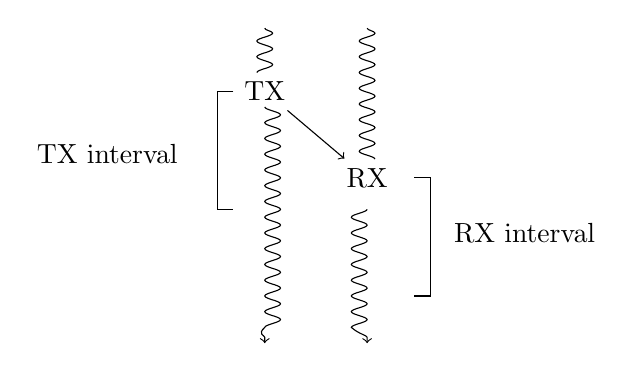
\begin{tikzpicture}
      \draw[->,decorate,decoration={snake,segment length=2mm, amplitude=1mm}]
        (0mm,0mm) -- (0,-5mm)
        (0mm,-8mm) node (TX) {TX} (0,-10mm) --
        (0mm,-40mm);
      \draw (-4mm,-8mm) -- (-6mm,-8mm) -- (-6mm,-23mm) -- (-4mm,-23mm);
      \draw (-20mm,-16mm) node {TX interval};

      \draw[->,decorate,decoration={snake,segment length=2mm, amplitude=1mm}]
        (13mm,0mm) -- (13mm,-16mm)
        (13mm,-19mm) node (RX) {RX} (13mm,-23mm) --
        (13mm,-40mm);
      \draw (19mm,-19mm) -- (21mm,-19mm) -- (21mm,-34mm) -- (19mm,-34mm);
      \draw (33mm,-26mm) node {RX interval};
      \draw[->] (TX) -- (RX);
    \end{tikzpicture}
    Intervals overlap; message is sent.
  \end{minipage}
  \begin{minipage}{35mm}
    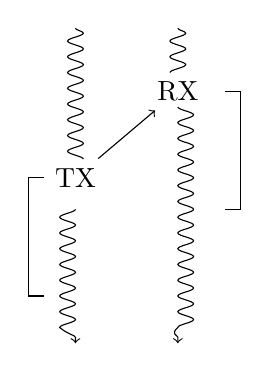
\begin{tikzpicture}
      \draw[->,decorate,decoration={snake,segment length=2mm, amplitude=1mm}]
        (0mm,0mm) -- (0,-16mm)
        (0mm,-19mm) node (TX) {TX} (0,-23mm) --
        (0mm,-40mm);
      \draw (-4mm,-19mm) -- (-6mm,-19mm) -- (-6mm,-34mm) -- (-4mm,-34mm);

      \draw[->,decorate,decoration={snake,segment length=2mm, amplitude=1mm}]
        (13mm,0mm) -- (13mm,-5mm)
        (13mm,-8mm) node (RX) {RX} (13mm,-10mm) --
        (13mm,-40mm);
      \draw (19mm,-8mm) -- (21mm,-8mm) -- (21mm,-23mm) -- (19mm,-23mm);
      \draw[->] (TX) -- (RX);
    \end{tikzpicture}
    Intervals overlap; message is sent.
  \end{minipage}
  \begin{minipage}{35mm}
    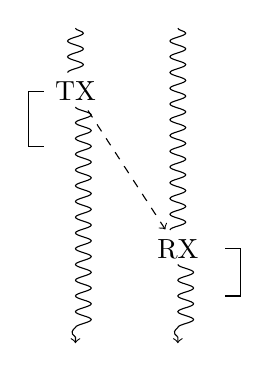
\begin{tikzpicture}
      \draw[->,decorate,decoration={snake,segment length=2mm, amplitude=1mm}]
        (0mm,0mm) -- (0,-5mm)
        (0mm,-8mm) node (TX) {TX} (0,-10mm) --
        (0mm,-40mm);
      \draw (-4mm,-8mm) -- (-6mm,-8mm) -- (-6mm,-15mm) -- (-4mm,-15mm);

      \draw[->,decorate,decoration={snake,segment length=2mm, amplitude=1mm}]
        (13mm,0mm) -- (13mm,-25mm)
        (13mm,-28mm) node (RX) {RX} (13mm,-30mm) --
        (13mm,-40mm);
      \draw (19mm,-28mm) -- (21mm,-28mm) -- (21mm,-34mm) -- (19mm,-34mm);

      \draw[->,dashed] (TX) -- (RX);
    \end{tikzpicture}\\
    Intervals do not overlap; no message can be sent.
  \end{minipage}
  \caption{Overlapping TX and RX intervals allow the message to be
    sent, regardless of which operation is ordered first.  If the
    intervals do not overlap then no message can be sent.}
  \label{fig:enforce:message_windows}
\end{figure}

\begin{algorithmic}[1]
  \If {The low-level interpreter has a bound interpreter}
    \If {The bound interpreter is not attempting to send a message}
      \State {Wait until it does so}
    \EndIf
    \State {Set $s'$ to the bound interpreter's outgoing message}
  \Else
    \State {Collect all outstanding unbound send operations as the set $s$}
    \State {Choose $s'$ non-deterministically from $s + \bot$}
    \If {$s' = \bot$}
      \State {Register the interpreter as a receiver of unbound messages}
      \State {Wait for the RX interval}
      \State {Unregister the interpreter as a receiver of unbound messages}
      \State {Collect all outstanding unbound send operations as the set $s$}
      \State {Select $s'$ non-deterministically from $s$}
    \EndIf
  \EndIf
  \If {$s'$ passes the side condition}
    \State {Discharge the message, unblocking the bound interpreter and moving to the Emul state}
  \Else
    \State {The plan has failed and the interpreter exits}
  \EndIf
\end{algorithmic}

The send operation is symmetric:

\begin{algorithmic}[1]
  \If {The low-level interpreter has a bound interpreter}
    \If {The bound thread is not attempting to receive a message}
      \State {Wait for it to do so}
    \EndIf
    \State {Set $s'$ to the bound interpreter's message receive operation}
  \Else
    \State {Collect all outstanding unbound receive operations as the set $s$}
    \State {Choose $s'$ non-deterministically from $s + \bot$}
    \If {$s' = \bot$}
      \State {Register the interpreter as a sender of unbound messages}
      \State {Wait for the TX interval}
      \State {Unregister the interpreter as a sender of unbound messages}
      \State {Collect all outstanding unbound receive operations as the set $s$}
      \State {Select $s'$ non-deterministically from $s$}
    \EndIf
  \EndIf
  \If {$s'$ passes the side condition}
    \State {Discharge the message, unblocking the bound interpreter and moving to the Succ state}
  \Else
    \State {The plan has failed and the interpreter exits}
  \EndIf
\end{algorithmic}

The behaviour when $s' = \bot$ is perhaps somewhat surprising: the
thread waits a little while and then selects a peer thread to
discharge the message with non-deterministically.  Meanwhile, all of
the other threads are simultaneously performing similar
non-deterministic choices.  The use of look-ahead nondeterminism means
that all of the threads will make these selections in a mutually
compatible way, so that there is no danger of A attempting to
discharge its message with B while B discharges with C.  The actual
implementation must resolve these constraints much more carefully, and
is discussed in detail later.

\subsubsection{Timeout balancing}
\label{sect:using:timeout_balancing}

Selecting the size of the various timeouts is important for
determining the likelihood of reproducing a bug and the overheads of
enforcing the patch.  SLI does so primarily dynamically, in response
to the program's observed behaviour.  I now consider briefly how these
timeouts should be set.

By far the most important timeouts are those which occur when unbound
interpreters synchronise, as bound-interpreter delays only happen when
the bug is already quite likely to reproduce, so assume for now that
those are the only two delays.  There are two such delays, one for
sending the first message and one for receiving it.  Call them $D_1$
and $D_2$.  Assume that the two CFGs occur randomly with rates $R_1$
and $R_2$.  Now the overhead introduced by the delays is $D_1.R_1 +
D_2.R_2$.  Ignoring side conditions, the bug will be reproduced if the
two CFGs occur such that the intervals on their initial message
operations overlap; in other words, if they occur with time $D_1 +
D_2$ of each other.  To put it another way, each occurrence of CFG 2
defines a window in the execution of size $D_1 + D_2$ such that the
bug will reproduce if CFG 1 starts anywhere in that window.  CFG 1
starts randomly with rate $R_1$, and so the probability of any given
instance of CFG 2 reproducing the bug is roughly $R_1(D_1 + D_2)$,
provided CFG 1 is sufficiently rare that we can neglect the
probability of two instances occurring in the window.  The expected
rate of bug reproduction is therefore $R_1.R_2.(D_1+D_2)$.  Some
simple algebra then allows us to show that if the desired overhead is
$k$, the reproduction rate will be

\begin{displaymath}
\alpha = k.R_2 + R_2.D_2(R_1 - R_2)
\end{displaymath}

So that if $R_1 > R_2$ the reproduction rate for a given level of
overhead is maximised by setting $D_2$ as large as possible, and
conversely if $R_2 > R_1$ the rate is maximised by setting $D_2$ as
small as possible.  In other words, if the total delay is fixed, it
should always all be apportioned to one side of the message operation.
{\Implementation} therefore keeps a counter of how many times the send
and receive sides of each message operation are attempted; if the send
operation has been attempted more times than the receive one then the
send operation delay is set to zero, and otherwise the receive delay
is set to zero.

\todo{Implementation currently sets the non-zero delay to some
  arbitrary constant plus a random fuzz; the next paragraph is an
  ambition.}

It now remains to set whichever of $D_1$ and $D_2$ is not fixed at
zero.  Assume without loss of that $D_2 = 0$.  {\Implementation} then
selects $D_1$ so as to achieve a particular level of overhead $k$ by
setting $D_1 = \frac{k - \frac{D_0}{R_2}}{R_1}$, where $D_0$ is an
estimate of the cost of entering the interpreter and then immediately
exiting.  This is not, in fact, a constant, due to the need to
sometimes interpret additional instructions as determined by the patch
strategy or to check side-conditions before considering a message
operation, but {\implementation} uses the constant time 100$\mu$s
anyway.\smh{hmm}

\subsubsection{Implementing non-deterministic choice in the Succ phase}

It might be that an instruction has several possible successors in the
control flow graph in the crash execution plan, and in that case the
interpreter must choose one of these successors using look-ahead
non-determinism.  This cannot be implemented in any
physically-realisable system, as it is non-causal, and so SLI must
emulate it.  SLI uses a power-set construction to do so.  Rather than
operating a single interpreter context, the actual implementation
maintains a set of low-level interpreter contexts, which individually
follow the abstract semantics given above, and interprets them all in
lock-step parallelism.  When one of these low-level interpreters needs
to perform a non-deterministic choice between $n$ possible values, the
high-level interpreter creates $n$ successor low-level interpreter
states, one corresponding to each possible outcome of the choice, and
inserts all of them into its current-state set.  They are then
interpreted in parallel until enough information is available to
resolve the earlier choice, at which point all but one of the threads
will exit and the interpreter can revert to ``single-threaded''
execution mode.  If a thread is bound when it performs a
non-deterministic choice then its bound thread must also be
duplicated, to ensure that the new thread has something to bind
to.\smh{Huh?  (I'm still suffering from lack of understanding of
  earlier text and terminology.)}

One subtlety here is that the original program's underlying
instruction can only be retired once, and so the high-level
interpreter must ensure that all low-level interpreters arrive at that
point in the execution cycle at the same time.  SLI actually enforces
a slightly stronger constraint, which is that every low-level
interpreter in a given high-level interpreter must be at the same
phase in the instruction execution cycle.  The semantics given above
is designed to ensure that this always possible.  The only phases for
which it is difficult are the message send and receive phases, which
are discussed in more detail in the next section.

\subsubsection{Concrete implementations of message send and receive}

The abstract semantics given above for message send and receive
operations is not realisable on any physical hardware as it relies on
non-causal nondeterministic lookahead.  Moreover, the power-set
construction used to resolve the non-deterministic Succ state is not
sufficient here as the message operation involves a sleep operation,
and hence has non-revocable externally visible side effects.  Solving
this problem requires the message operation to be ``turned inside
out'', restructuring it into a fragment which occurs before the sleep
and another fragment which occurs after it with the remaining
non-determinism confined to the two fragments.  The resulting message
receive operation looks like this:

\todo{Urk; big wall of algorithm.  This cannot be the best way of
  describing this.}

\begin{algorithmic}[1]
  \State {$lls \gets $ the set of currently-active low-level interpreter states}
  \State {$newLls \gets $ an empty set of low-level interpreter states}
  \For {$l$ in $lls$}
    \If {$l$ does not receive any messages}
      \State {Move $l$ from $lls$ to $newLls$ without changing it}
    \ElsIf {$l$ has a bound thread}
      \If {$l$'s bound thread has exited}
        \State {$l$ exits as well; remove it from $lls$ without adding it to $newLls$}
      \ElsIf {$l$'s bound interpreter's sending-bound-message flag is set}
        \If {The bound interpreter's outgoing message passes any side condition}
          \State {Move $l$ from $lls$ to $newLls$}
          \State {Clear the bound interpreter's sending-bound-message flag}
        \Else
          \State {$l$ exits; remove it from $lls$}
        \EndIf
      \Else
        \State {Set $l$'s receiving-bound-message flag}
      \EndIf
    \Else \Comment{Unbound receive}
      \For {$s$ registered unbound senders}
        \If {$s$'s outgoing message passes the side condition}
          \State {$l' \gets $ duplicate $l$}
          \State {$s' \gets $ duplicate $s$}
          \State {Bind $l'$ and $s'$ together}
          \State {Insert $l'$ into $newLls$}
          \State {Insert $s'$ into $s$'s high-level interpreter's active low-level interpreter list}
        \EndIf
      \EndFor
      \State {Register $l$ as an unbound receiver}
      \State {Set the minimum delay to the receive operation's delay, if it is currently less than that.}
    \EndIf
  \EndFor

  \If {$lls$ is empty}
    \State \Return
  \EndIf

  \State {$end \gets now() + bound\_delay$}
  \If {There is a minimum delay}
    \State {Sleep for the minimum delay}
  \EndIf

  \While {There are bound receives in $lls$ and $now() < end$}
    \State {Wait for some bound receive to complete, or for the current time to pass $end$}
    \For {$l$ performing bound receives in $lls$}
      \If {$l$'s bound thread has exited}
        \State {Remove $l$ from $lls$}
        \State {$l$ exits}
      \ElsIf {$l$'s receiving-bound-message flag is clear}
        \State {Remove $l$ from $lls$}
        \State {Add $l$ to $newLls$}
      \Else
        \State Continue waiting
      \EndIf
    \EndFor
  \EndWhile

  \For {$l$ in $lls$}
    \If {$l$ is registered as an unbound receiver}
      \State {Unregister $l$ as an unbound receiver}
    \EndIf
    \If {$l$'s receiving-bound-message flag is set}
      \State {Exit $l$} \Comment{Receiving bound message failed}
    \ElsIf {$l$ is unbound}
      \State {$l$ must have been attempting an unbound receive which failed, so it exits}
    \Else
      \State {Add $l$ to $newLls$}\Comment {Receive succeeded}
    \EndIf
  \EndFor
\end{algorithmic}

For clarity, I have omitted the synchronisation on the various
interpreter-internal structures.  The send algorithm is symmetrical,
simply replacing the word ``receive'' with the word ``send'' and vice
versa.  There are a couple of features to note in this algorithm:

\begin{itemize}
\item
  If there are any unbound message operations then it waits for the
  whole of that message's delay, even if some other interpreter which
  might match the operation arrives.  This reflects the semantics
  already discussed in which any message operation will synchronise
  will all other matching operations in its window.  On the other
  hand, it can lead to poor performance, and the slight loss of
  correctness from ending the wait early is very rarely important.
  \todo{Say more.}
\item
  When interpreters are bound together both interpreters are
  duplicated.  This means that the original interpreter is left in the
  unbound send state, and can therefore synchronise with any
  additional interpreters which might arrive.
\item
  Bound messages use a different delay strategy to unbound ones.  This
  is because bound operations fail in different ways.  By
  construction, a bound interpreter will eventually either exit or
  perform all planned message operations and so it might appear that
  bound operations should never hit their timeout, and that is indeed
  the common case.  It is, however, possible, albeit very rare, for
  {\technique} enforcers to introduce a deadlock if they interact
  badly with the program's existing synchronisation structure.  These
  timeouts avoid that issue.  \todo{Actually, now I think about it, I
    don't think that deadlock is actually possible, but I don't want
    to have to prove that, so maybe just pretend that it is.}
\end{itemize}

Note that the side condition is evaluated as the message is being
discharged, while the two interpreters are merged.  \todo{This is
  incomprehensible, which is a pity because it's also quite
  important.}\smh{Yes, I agree!! (or more precisely, I half agree)} It
is possible to imagine an alternative implementation in which
discharging the message copies enough state from the transmitting
interpreter to the receiver to allow the condition to be evaluated
locally in the receiver after the interpreters have been
unmerged\footnote{Or, conversely, one where state is copied from the
  receiver to the transmitter and the side-condition evaluated in the
  transmitter after transmission.}.  This would reduce the size of the
synchronised section and so would appear, on the face of it, to offer
greater parallelism, and hence potentially better performance.
Unfortunately, it does not work.  To illustrate the problem, consider
again the example shown in Figure~\ref{fig:using:example_hb_graph}.
One thread modifies a shared structure while another thread reads it,
and the program will crash if the two threads happen to be operating
on the same structure at the same time.  Suppose that the read thread
runs far more often than the write one and that there are many
instances of the structure.  The timeout balancing logic will quickly
reduce the delay on the read side's first message send to zero and
increase the delay on the write side's first message receive to
compensate.  Now, when the write interpreter does run it will stop
just before \verb|l9| waiting for a matching read interpreter to
arrive.  \smh{I'm kind of with you until about here, but the bit after
  is complete gobbledegook to me.} By hypothesis, many such
interpreters will arrive, as the read thread runs more often than the
write one.  In the alternative design, the side condition can only be
evaluated in the receiving interpreter once the message operation is
complete.  In this case the receiving interpreter is the write thread,
and so every read interpreter will be forced to bind to the write
thread.  Only one interpreter can be bound to the write thread at any
one time, and so satisfying these later attempts to bind will force
the write interpreter to be duplicated many times.  Because of timeout
rebalancing, the read interpreter will proceed from \verb|l2|
immediately and quickly reach \verb|l5|, where it has to receive a
message from \verb|l9|.  At this point, there are two possible
outcomes:

\begin{itemize}
\item
  The read interpreter is delayed at \verb|l5| waiting for the message
  from \verb|l9|.  The write interpreter is still waiting in case any
  other threads reach \verb|l2| and attempt to synchronise with it,
  and so this might potentially be a rather long delay.  Since the
  read thread runs far more often than the write thread, this will
  have a very large performance impact.  Worse, it will probably be
  pointless: there are, by hypothesis, a large number of instances of
  the structure which is being examined, and so, with high
  probability, the write thread will be modifying a different one.
  When the write interpreter does finally escape from its receive
  delay and evaluate the side condition it will discover that the
  filter fails, and so the write thread will exit.  The read thread
  will then discover that its bound thread has exited and be forced to
  exit as well.  The crash enforcement plan will therefore not
  complete and the bug is highly unlikely to reproduce.
\item
  The thread is not delayed at \verb|l5|.  It never receives the
  message from \verb|l9| and must therefore exit without completing
  the plan, so is unlikely to reproduce the bug.  The write thread's
  high-level interpreter will then accumulate a collection of
  low-level threads which have bound to exited read threads and which
  will themselves immediately exit.
\end{itemize}

Neither outcome helps to reproduce the target bug.

By contrast, in the scheme used by SLI, the read thread is able to
evaluate the side condition at \verb|l2| and will therefore only bind
to write threads which modify the structure which it is reading.  That
means that the thread can be delayed a relatively long time at
\verb|l5| without fear of apocalyptic performance damage, and so the
bug will reproduce relatively easily.

One further optimisation, not shown here but implemented in
{\implementation}, avoids redundantly duplicating low-level
interpreter contexts in the common case that a message operation is
discharged precisely once.

\subsubsection{Starting new low-level interpreters}

The high-level interpreter is responsible for starting new low-level
interpreters as the program under test moves through CFG nodes which
are marked as entry point nodes.  This might be because the program
has just reached one of the interpreter entry point instructions,
already discussed in the discussion of building patch strategies.  It
might also be because the program has reached an entry point while
running under the interpreter, in which case the high-level
interpreter must start another low-level interpreter to handle the new
CFG.  This can happen if the one of the CFG fragments is
cyclic\editorial{Or as cyclic as the unrolled CFG fragments ever
  get...} and re-enters itself, or if two of the CFG fragments
overlap.  {\Implementation} handles either case by spawning additional
low-level interpreters.  After starting a new low-level interpreter
the high-level interpreter must sample the value of any needed
processor registers and evaluate any appropriate side-conditions, as
already discussed.  The new low-level interpreter can then be added to
the high-level interpreter state and interpretation proceeds as
already discussed.

\subsubsection{The await-bound-thread-exit state}

When a thread completes its plan, it is sometimes useful for it to
wait for its bound thread to exit before proceeding.  This is because
the crash summary from which the plan is generated does not have
complete information on the structure of the program and can miss
relevant stores which happen after the write-side {\StateMachine}
completes.  If the last edge in a happens-before graph is from memory
access A to memory access B, that usually means that A is a store and
B is a load and B must load the value stored by A.  That means that,
not only must B happen after A, but B must happen before any other
writes to the memory location modified by A.  If there were other
stores to that location in the crash summary then the happens-before
graph would include additional edges to ensure that that happens, but
if there are stores outside of the analysis window then it will not.
For instance, suppose that the write thread looks like this:

\begin{verbatim}
while (1) {
l1:  *x = 5;
l2:  *x = 7;
     <something_complicated>
}
\end{verbatim}
\smh{Indent}

And the read thread looks like this:

\begin{verbatim}
l3: a = *x;
l4: b = *x;
    crash if a != b;
\end{verbatim}

This program is clearly buggy.  One way of reproducing this bug would
be to interleave instructions as \verb|l1|, \verb|l3|, \verb|l2|,
\verb|l4|, and SLI will discover this interleaving as the
happens-before graph show in Figure~\ref{fig:enforce:await_exit_hb}.
The algorithm described so far will be sufficient to enforce this
graph (assuming that the two fragments of code shown can actually
execute in parallel) but may still struggle to reproduce the bug.
This is because the generated happens-before graph is incomplete: it
misses the edge from \verb|l4| to \verb|l1| in the next iteration of
the loop.  If the loop completes and reaches the store at \verb|l1|
before the load \verb|l4| completes then the bug will not reproduce
even though the happens-before graph was successfully enforced.  The
workaround for this problem is simple: if a low-level state ends with
a successful message send then the sending thread is not allowed to
execute any further instructions until the receiving thread has either
completed a further instruction or has itself exited.  This ensures
that activity beyond the analysis horizon cannot prevent bug
reproduction, and, because it only happens when the plan is mostly
complete, and thus very rarely, it has very low performance overhead.

\begin{figure}
\begin{tikzpicture}
\node[CfgInstr] (l1) {l1};
\node[CfgInstr, below = of l1] (l2) {l2};
\node[CfgInstr, right = of l1] (l3) {l3};
\node[CfgInstr, below = of l3] (l4) {l4};
\draw[->] (l1) -- (l2);
\draw[->] (l3) -- (l4);
\draw[->,happensBeforeEdge] (l1) -- (l3);
\draw[->,happensBeforeEdge] (l3) -- (l2);
\draw[->,happensBeforeEdge] (l2) -- (l4);
\end{tikzpicture}
\caption{Happens before graph for the await-bound-exit example.}
\label{fig:enforce:await_exit_hb}
\end{figure}

\smh{Is this important?  Why?}

\subsection{Combining multiple enforcers}
\label{sect:enforce:combine_enforcers}

The initial static analysis and symbolic execution phase can generate
a large number of false positives, and it would be extremely tedious
to have to test each one independently.  {\Implementation} therefore
includes a mechanism for enforcing multiple bugs at once.

\todo{How does this work?  Actually very simple: you generate
  mostly-independent plans for each VC, and then have the high-level
  interpreter start low-level interpreters for each of them as
  appropriate.  The only time it gets complicated is when you have
  contradictory happens-before graphs, but I don't have a good story
  for that yet.}

\subsection{Run-time considerations}

Evaluating side conditions\smh{I'm not sure calling these ``side
  conditions'' helps... is there a better phrase/term?} is not always
completely trivial, even once all of the inputs are available.  In
particular, $LD(addr)$ expressions require a moderate amount of care.
These are defined to return the contents of memory at a particular
address.  The problem is that the address might turn out to be a bad
pointer, and it is important for the enforcer not to cause the program
to crash in that case.  {\Implementation} solves this problem by
simply catching page faults generated while evaluating side
conditions.  If any such faults occur then the relevant low-level
interpreter state is considered to have failed.  This is not always
ideal from the point of view of reproducing the bug, but avoids
spuriously crashing the program under test.

\todo{Another major approximation: $LD$ is supposed to return the
  initial contents of memory, but that's not necessarily available.
  The enforcers evaluate $LD$s as soon as they can evaluate the
  address to be loaded, which is pretty much as good as you can get,
  but it's still not \emph{quite} right.}

\todo{Why do we sometimes end up dereferencing pointers which the
  program never does? Answer: because the placement stuff sometimes
  ends up pulling validation over program control flow, which makes it
  easier to implement and easier to fast-out of the enforcer, but
  risks introducing these bad dereferences.}

\section{Fixing bugs using global locks}
\label{sect:fix_global_lock}

In addition to finding bugs, SLI can also be used to fix them.  The
basic approach here is to binary patch the program to introduce a new
global lock covering the program's relevant instructions, preventing
them from executing in parallel and hence preventing the bug from
occurring (assuming that the relevant instructions have been correctly
identified).  The relevant instructions are duplicated into a binary
patch, unrolling loops and tracing across function boundaries in a way
which reflects the function inlining and loop unrolling performed
during the initial CFG generation phase, and the duplicates modified
to acquire and release the lock at appropriate points.  The original
program is then patched to branch to the duplicates when necessary.

The first step in producing such a fix is correctly identifying the
instructions which must be included in the critical sections.  These
will be roughly a subset of the instructions involved in the
control-flow graphs associated with \StateMachines; a ``subset''
because some instructions in the CFG do not need to be protected, and
``roughly'' because some instructions not in the CFG will also be
included in the critical section.

\todo{Already explained this once in the context of building crash
  summaries and enforcers!}

As an example of the former, consider a program like this:

\begin{verbatim}
read_side() {
    ptr = complicated_local_calculation();
    dptr = *ptr;
    if (dptr != NULL) {
       dptr = *ptr;
       *dptr = 5;
    }
}
write_side() {
    ptr = complicated_local_calculation();
    *ptr = NULL;
}
\end{verbatim}

Here, the read thread computes some pointer using entirely local
operations, loads from it once and then, if the result is
non-\verb|NULL|, loads from it again and uses the resulting pointer.
Meanwhile, the store thread sets a potentially coincident memory
location to \verb|NULL|.  The read thread clearly has a potential
time-of-check, time-of-use race bug.  The {\StateMachines} generated
by {\technique} will include the buggy code itself but might also
include part or all of \verb|complicated_local_calculation()| and a
side-condition which requires the two pointers to match up.  This
extra information is useful when analysing the bug
(\S\ref{sect:using:check_realness}) or when attempting to reproduce it
(\S\ref{sect:using:reproducing_bugs}) but cannot be used by this kind
of instruction-level fix\footnote{But see future work for a possible
  alternative scheme which would make use of it.}, so including it in
the fix is unhelpful and would tend to lead to unnecessarily large
critical sections.  The fix generating process must therefore select a
useful subset of the instructions in the control-flow graph.

The approach taken here is simple:

\begin{itemize}
\item
  Extract all of the happens-before edges from the bug summary's
  verification condition.  These entirely capture the
  instruction-interleaving parts of the bug to be fixed, and, since
  instruction-interleaving is the only thing which can be influenced
  by this type of patch\smh{As opposed to?}, the resulting set of
  edges contains all of the useful information in the condition.
\item
  Identify all of the CFG nodes which are mentioned in one of those
  happens-before edges.
\item
  Trim the CFG such that every path starts and ends in one of those
  mentioned nodes.  All such paths will be included in a critical
  section, and so no such paths will be permitted to execute in
  parallel.
\end{itemize}

In this way the CFG is restricted to just those instructions which are
involved in the interleaving which is to be prevented.

Note that this is not guaranteed to produce an optimal selection of
critical sections, in the sense that sections can sometimes be larger
than is strictly necessary.  Consider, for example, a program with the
same read side as the previous example but a write side in which the
pointer is assigned to twice:

\begin{verbatim}
write_side() {
    ptr = complicated_local_calculation();
    *ptr = NULL;
    *ptr = NULL;
}
\end{verbatim}
    
There are now two obvious ways of protecting this program:

\begin{itemize}
\item
  Place both loads in the read side in a single critical section and
  both stores in the write side in another one.
\item
  Place both loads in the read side in a single critical section, but
  give each store in the write side its own critical section.  In
  other words, drop and re-acquire the lock in between the two stores.
\end{itemize}

Both approaches correctly eliminate the bug, but they will have
different performance characteristics.  In particular, dropping and
re-acquiring the lock reduces the size of the critical section, which
might improve concurrency and reduce starvation, but imposes higher
overheads due to the greater number of lock operations.  In principle
the happens-before graph implicit in the verification condition
contains enough information to determine whether dropping the lock is
safe, but, in this mode\smh{??You mean ``bug fixing mode''??}, SLI
does not make use of this information, and always uses the former
strategy\footnote{But see~\ref{sect:fix_from_drs} for a mode in which
  it can use the other approach.}.

Once the relevant fragments of CFG have been identified, {\technique}
must examine the machine code of the original program and effectively
re-compile it so as to introduce the necessary synchronisation
operations.  This is more complicated than it might at first appear,
most importantly because the CFG fragments to be protected are taken
from the {\StateMachines} rather than from the original program, and
the two graphs do not match up precisely.  There are two interesting
cases:

\begin{itemize}
\item
  The program CFG might include edges which are not present in the CFG
  to be protected.  In that case, the patch must ensure that the lock
  is correctly released when one of these edges is traversed before
  returning to the unmodified program.
\item
  The CFG to be protected might include edges which are not present in
  the program CFG, due to loop unrolling.  In that case, the patch
  must, in effect, consider every possible path through the graph and
  ensure that the lock is not dropped until they have all completed.
\end{itemize}

As a further complication, the patch might need to protect multiple
CFG fragments, and these fragments might in some cases overlap.  It
must then ensure that the lock is held until every fragment has
completed, without ever allowing a thread to acquire the lock twice
and hence deadlock against itself.  Finally, the patch might also need
to include additional instructions which are not part of any CFG
fragment if the patch strategy (discussed in
Section~\ref{sect:enforce:assign_entry_points}) added extra
instructions to the $Cont$ set\smh{blurk!}.  The result is that the
code in the duplicated patch fragment is not quite an exact match for
that in the original program, even ignoring the additional lock
acquire and release operations.

The simplest way of thinking about this is to first augment the
machine code semantics so as to include the necessary additional
information, so that enforcing the necessary locking discipline is
simply a matter of interpreting this enhanced semantics, and to then
partially evaluate this interpreter to produce machine code in the
original semantics.  The output of this partial evaluator then forms
the bulk of the fix.

\smh{This is a strange way of thinking about it (to me at least).}

The state of a thread in the augmented semantics consists of all of
the state of a thread in the original semantics, including things like
the per-thread processor registers and instruction pointer, plus a
small amount of additional state:

\begin{itemize}
\item $checkForEntry$ -- a flag indicating whether the thread needs to
  check whether it has entered any additional CFG fragments.
\item $locked$ -- a flag indicating whether the thread currently holds
  the patch lock.\smh{Ugly}
\item $\mathit{cfgNodes}$ -- a set of nodes taken from the CFG fragments
  indicating which instructions the thread might currently be
  executing.  This might be empty if the thread is currently executing
  one of the additional instructions in the patch strategy's $Cont$
  set.
\end{itemize}

The $Patch$ instructions in the patch strategy are then treated as
transitions from the normal program semantics into the augmented
semantics.  The initial augmented state is then the state of the
original program at the entry point, plus:

\begin{itemize}
\item $checkForEntry$ is true.
\item $locked$ is clear.
\item The set of CFG nodes is empty.
\end{itemize}

Conceptually, the patch then takes control of the program and
interprets it using the augmented semantics.  Such an interpreter
would be quite simple:

\begin{itemize}
\item[\textbf{CheckForEntry}] If the $checkForEntry$ flag is set then the
  interpreter would examine the current call stack and the possible
  set of CFG fragment entry points to determine whether any new CFG
  fragments have started.  If so, the relevant CFG nodes added to
  $\mathit{cfgNodes}$.  In either case, $checkForEntry$ is cleared.
\item[\textbf{Return}] The interpreter would then consider returning
  to the program's normal semantics.  This is safe if $\mathit{cfgNodes}$ is
  empty and the instruction pointer is not part of the $Cont$
  set\footnote{Note that the thread is guaranteed not to be holding
    the lock at this point.}  The transfer itself is quite simple:
  just branch to the relevant instruction pointer in the original
  program.
\item[\textbf{Lock}] The interpreter now acquires the lock, provided
  that $\mathit{cfgNodes}$ is non-empty and $locked$ is currently clear,
  setting $locked$ as it does so.
\item[\textbf{Issue}] The interpreter emulates the program's original
  instruction, using the un-augmented semantics, writing back any
  required changes to memory or the process registers.  This will
  include updating the thread's instruction pointer, and the
  interpreter can then easily use this to determine which CFG nodes
  the thread might execute next and hence the new value of $\mathit{cfgNodes}$.
\item[\textbf{Unlock}] Finally, the interpreter would check whether it
  needs to release the lock.  It should do so whenever $locked$ is set
  and $\mathit{cfgNodes}$ is empty, clearing $locked$ as it does so.  The
  interpreter then returns to the \textbf{CheckForEntry} state and the
  cycle begins again.
\end{itemize}
  
Such an interpreter would correctly enforce the desired lock
discipline, in the sense that the lock would always be held whenever
the program executes one of the CFG fragments which are to be
protected, but would have two major disadvantages:

\begin{itemize}
\item Emulating machine code instructions is usually quite slow, which
  could lead to unnecessarily high performance overhead.
\item Instruction emulators are extremely complex pieces of code, and
  so it is difficult to have complete confidence that the fix does not
  change the program's behaviour in unintended ways.
\end{itemize}

Both of these disadvantages are shared with the use of an interpreter
in crash enforcers, but are far more serious here, as crash enforcers
are intended as temporary debug aids whereas the generated fixes might
be deployed in production environments for significant amounts of time
before a real fix becomes available.  {\Technique} therefore refines
on this interpreter scheme by partially evaluating the
interpreter\needCite{} back into machine code in the unaugmented
semantics, and it is the result of this partial evaluation which forms
the body of the patch.  In effect, the augmented state is encoded into
the instruction pointer, allowing the patch to emulate the interpreter
without it ever needing to be present.  Updating part of the augmented
state then becomes a simple branch instruction.  None of the augmented
interpreter state is ever stored in memory or processor registers,
minimising the unnecessary perturbation of the program.

In a little more detail:

\begin{itemize}
\item The \textbf{CheckForEntry} state partially evaluates to a stack
  context validation tree, as discussed in \todo{...}.  The leaves of
  this validation tree will contain branches to augmented instructions
  in the \textbf{Return} state with an appropriately-augmented
  $\mathit{cfgNodes}$ set\editorial{The \textbf{Return} state will then
    immediately discover that $\mathit{cfgNodes}$ is non-empty and move to
    \textbf{Lock}, but actually saying that makes the parallels with
    the interpreter a bit less obvious.}.

  The current (unaugmented) instruction pointer and current $\mathit{cfgNodes}$
  set usually place significant constraints on the set of entry points
  which the thread might currently be executing, and so the validation
  tree can often itself be partially evaluated to determine precisely
  which CFG nodes must be executed next.  In that case, the tree is
  replaced with a simple branch instruction.
\item \textbf{Lock} and \textbf{Unlock} states partially evaluate to a
  possible call to a lock acquire or release function, as appropriate,
  followed by a simple branch to the next state.
\item \textbf{Return} states partially evaluate to either a branch
  back to the original program code, if $\mathit{cfgNodes}$ is empty and the
  address to return to is not in the patch strategy's $Cont$ set, or a
  branch to the \textbf{Issue} state otherwise.
\item Most of the time, the \textbf{Issue} state partially evaluates
  to the relevant instruction of the original program which can
  execute in the augmented semantics without modification.  The main
  exceptions are instruction pointer-relative data addressing modes,
  which must be re-encoded to reference the correct data relative to
  the new instruction pointer, and control flow instructions, which
  are discussed below.  Assuming that this is not a control flow
  operations, the state updates $\mathit{cfgNodes}$ to contain all of the CFG
  nodes which are successors of current members of $\mathit{cfgNodes}$ and
  whose instruction pointer matches that of the desired successor
  instruction and then returns to state \textbf{CheckForEntry}.
\end{itemize}

Partially evaluating one augmented state produces a small fragment of
machine code and a set of successor augmented states.  Building the
patch then amounts to initialising a queue of states with the initial
state and then iteratively selecting a state from the queue, partially
evaluating it, placing the new states in the queue, and continuing
until no further states need to be generated.  The machine code
fragments can then be stitched together to produce the final patch.

As a minor optimisation, {\implementation} eliminates branch
instructions which target the immediately following instruction.

One non-obvious complication here is that calling the lock acquire and
release functions is not completely trivial, due to the presence of a
stack red zone in the AMD64 ABI\needCite{}.  This is a 128 byte region
immediately below the stack pointer which is available for program
use.  It is important that the generated patch not corrupt values in
this region, which means that the patch cannot save clobbered
registers by simply pushing them on the stack as a patch to an i386
program might.  It must instead first clear the red zone from the
stack by adjusting the RSP register and then restore it later before
executing any instructions from the original program which depend on
it.  At the same time, we would like to avoid redundant clearing and
restoring the red zone more often than is strictly necessary.
{\Implementation} therefore extends the augmented state with an
additional field, $redzone$, indicating whether the red zone has been
cleared, allowing red zone clearing to be performed precisely when
necessary.

\todo{Move this para to be later.}\smh{Yes} One concern here might be
that modifying the program's stack in this way might confuse another
thread which is simultaneously examining the stack.  Such cross-stack
accesses are rare in most programs anyway, and in any case are handled
correctly for correct programs here because the modified stack pointer
never escapes into any of the original program's code.  This means
that the modifying thread will not be able to determine that
additional stack space has been allocated, and so will only be able to
tell that the stack has been modified if it is accessing what is, as
far as it can tell, memory past the end of the stack.  This is not
allowed by the ABI, and so correct programs will not do it.  You might
suspect that operating system introspection services such as
\verb|ptrace| would allow the remote thread to tell that the stack
pointer register has been modified, but this is highly unlikely, at
least on modern versions of Linux, which prohibit one thread in a
program from calling \verb|ptrace| on another\needCite{}.  The remote
thread would therefore need to coordinate the \verb|ptrace| operation
with another process, and such an unlikely configuration is ignored
here.  {\Technique} does not claim to be able to protect programs
which are actively trying to avoid its protection, and so the fact
that the generated patches misbehave on some actively malicious
program is not a problem such behaviour is sufficiently rare in real
programs.  \todo{Signal handlers can also leak the fact that we've
  extended the stack.  Also need to talk about why there's no
  realistic risk of running out of stack space here.}

Control flow operations are not completely trivial to represent in
this model.  Direct control flow, where the target of the control flow
transfer is immediately apparent from the instruction itself, is
relatively easy and can be handled by comparing the target address to
the possible successors of all of the CFG nodes in $\mathit{cfgNodes}$ and
generating a new successor state with $\mathit{cfgNodes}$ appropriately
updated.  Indirect control flow is more difficult and requires run
time validation of the target address.  There are three main cases to
consider: indirect jumps, indirect calls, and return instructions.

\paragraph{Indirect jump instructions,} which simply set the instruction pointer
to a calculated value\smh{Not a sentence.}.  In order to partially
evaluate these states {\technique} must examine all of the successors
of nodes in the $\mathit{cfgNodes}$ set and segregate them by their instruction
pointer.  The code generated for the state will compare the target of
the branch instruction to each such instruction pointer in turn and,
when one matches, jump to an augmented instruction with an appropriate
$\mathit{cfgNodes}$ set.  If none match then the patch moves on to consider
instructions in the patch strategy's $Cont$ set\smh{This is a detail
  that doesn't matter at a certain level of abstraction; you need to
  separate the idea/algorithm from the combined code you've written.},
comparing the generated branch target to each in turn and branching to
an appropriate augmented instruction if any match.  Finally, if none
of those match, the patch can exit the augmented semantics by directly
branching to the computed branch target, dropping the lock first if
necessary.

A further complication is that computing the branch target might
itself involve reading from memory, and this access might itself race.
It would be unfortunate if this led to the patch branching to the
wrong place, and so the patch must first capture the computed branch
target to a register\footnote{In more detail, the concern is that the
  target address might change from one instruction which must be
  protected to another instruction which must be protected, and the
  patch must ensure that the race does not cause it to prematurely
  drop the lock.  It does not matter which protected path the patch
  ultimately follows, provided it follows one of them}.  This means
that the register must first be saved somewhere, so that it can be
restored later, which in turn means that the red zone must be cleared.
Both of these operations must be undone later.  This is recorded by
setting the $redzone$ field of the augmented state to the special
$popreg$ value.

Of course, setting $redzone$ does not actually help if the patch is
about to return to the unaugmented program, as in that case $redzone$
will never be examined.  The patch must then restore the register used
to capture the computed branch target, restore the red zone, and
finally branch to the computed target, without using any additional
registers.  The scheme used by {\implementation} uses a machine code
fragment like this:

\begin{verbatim}
xchgq %rdi, (%rsp) ; Restore rdi and set the next instruction address
ret $0x80          ; Restore the red zone and branch to the next instruction
\end{verbatim}

\todo{Not sure how interesting this actually is, but it took me bloody
  ages to figure out how to do it, which suggests there should
  probably be something about it in here.}  Here, \verb|rdi| is the
register used to store the computed branch target, the old value of
\verb|rdi| was stored to the top of the stack before the branch was
computed, and \verb|0x80| is the size of the red zone.  In this
sequence, the \verb|xchgq| instruction swaps the top of the stack with
\verb|rdi|, restoring the old value of \verb|rdi| and setting the top
of the stack to the target of the branch and the \verb|ret|
instruction then branches to this location and removes the top
\verb|0x80| bytes from the stack, restoring the red zone.  The
sequence therefore correctly implements the desired behaviour.

It does, however, have some unpleasant performance implications.  In
particular, the \verb|ret| instruction does not match with any
\verb|call| instruction, which can be extremely difficult for
processor branch prediction units to handle\needCite{}, and if this
leads to a branch misprediction then performance will be quite poor.
Unfortunately, there is no other way of achieving the desired
behaviour with the x86 instruction set without using additional
registers, because the instruction and stack pointers must be modified
simultaneously and \verb|ret| is the only instruction capable of doing
so.  Modifying the instruction pointer before the stack pointer is
obviously unprofitable, as modifying the instruction pointer means
that we lose control of program execution and therefore never get the
chance to perform the stack pointer modification.  Modifying the stack
pointer first, though, sounds like it might be an effective strategy.
The resulting fragment of code might look like this:

\begin{verbatim}
lea 0x80(%rsp), %rsp   ; Restore the red zone
xchgq %rdi,-0x88(%rsp) ; Save the branch target and restore rdi
jmp -0x88(%rsp)        ; Perform the branch
\end{verbatim}

Executed in isolation, this code correctly sets all three registers
(\verb|rdi|, the stack pointer, and the instruction pointer), and
avoids damage to the branch prediction units.  In a program running on
most Unix-like operating systems, however, it contains a dangerous
race with signals.  The target of the branch instruction is stored
\verb|0x88| bytes below the stack pointer, just outside of the red
zone.  If the program receives a signal immediately before executing
the \verb|jmp| instruction then this is precisely the location at
which the signal handling stack frame will be constructed, clobbering
the branch target.  When the signal handler returns the program will
almost certainly crash.  Avoiding this issue is impossible without
forcing the program to use a dedicated signal stack, which is
extremely fragile without cooperation from the program\footnote{An
  alternative scheme would be to just disable signals during the
  critical section.  This does not work, as the signal disposition
  must be restored when the program resumes, which requires a system
  call and hence the use of registers, which brings us back to the
  original problem.}.

\smh{This is all fine, but it is a detail that probably doesn't
  deserve the best part of a page!  Focus, select, highlight,
  abstract.}

\todo{Maybe explain why I'm happy to use the GS trick in the enforcers
  but don't want to do so here?}

\paragraph{Indirect call instructions,} which are similar to indirect jumps
except that they also store the current instruction pointer to the
stack\smh{Not a sentence.}.  The issues involved here are similar,
except that the patch must store the return address in addition to
maintaining the stack pointer and branching to an appropriate
location.  If the interpreter is to continue then this can be
accomplished by setting $redzone$ to another special value,
$finishCall(return\_address)$.  Otherwise, the exit sequence can be
modified slightly:

\begin{verbatim}
mov %rdi, 0x80(%rsp) ; Store next instruction address
mov 0(%rsp), %rdi    ; Restore RDI
lea 0x80(%rsp), %rsp ; Restore red zone
call *0(%rsp)        ; Call target function
jmp return_address   ; Return to original program
\end{verbatim}

\todo{At the moment the implementation just uses the silly ret thing.
  I should switch it over to that sequence, because it's awesome.}

This perhaps requires some additional explanation:

\begin{itemize}
\item \verb|mov %rdi, 0x80(%rsp)|.  This stores the address which we
  need to call into \verb|0x80(%rsp)|.  \verb|0x80| is the size of the
  red zone, and so once the red zone has been cleared this will be
  \verb|0(%rsp)|.
\item \verb|mov 0(%rsp), %rdi|.  This restores the value of
  \verb|%rdi| from the top of the stack.
\item \verb|lea 0x80(%rsp), %rsp|.  This restores the program's
  original red zone.  The address which is to be called is now at
  \verb|0(%rsp)|.
\item \verb|call *0(%rsp)|.  The effect of this instruction is
  somewhat complicated: it sets the instruction pointer to the initial
  contents of \verb|0(%rsp)|, then sets \verb|0(%rsp)| to the address
  of the next instruction, and then decrements \verb|%rsp| by eight
  bytes.  This means that the target function will be invoked with the
  desired stack pointer and its return address set to the \verb|jmp|
  instruction.
\item \verb|jmp return_address|.  This runs once the called function
  returns and immediately branches to the instruction after the
  indirect call instruction.
\end{itemize}

This means that the indirect branch is correctly emulated, provided
that the program never explicitly examines return address addresses on
its stack, and the processor's branch predictor state is correctly
maintained.  The potential race with signals is avoided completely
because the address which is to be branched to is stored within the
program's red zone.  Modifying the red zone is safe because we know
that the \verb|call| instruction is itself about to overwrite the
modified location\footnote{The exception is if another thread is
  simultaneously examining this thread's call stack, in which case we
  have potentially introduced an additional race condition.  Such a
  race condition is implausible given common programming practices and
  I ignore the possibility here.}.

\paragraph{Return instructions,} which pop an address off of the stack
and return to it\smh{Not a sentence}.  If the $cfgNode$ set is
currently non-empty then this is very simple because, by construction,
when the $cfgNode$ set is non-empty the program's call stack must
match the call stack in the CFG nodes.  That means that the return
instruction can be partially evaluated without needing to examine the
actual contents of the stack, and the only instruction which actually
needs to be emitted is \verb|lea 8(%rsp), %rsp|, which pops the return
address off of the stack and discards the result.  \todo{Actually need
  a couple more side-conditions on that, but they're not terribly
  interesting and would just confuse things a bit.}

\todo{But that branch means that you end a function with a jump rather
  than a ret, which is going to screw your branch predictor despite
  our best efforts.  That's particularly sad given that if the match
  call was part of the patch then the address on the top of the stack
  will be the address which we're branch to anyway.  Need to think
  harder about that.}

An empty $cfgNode$ set is slightly more difficult to handle, but only
slightly.  In this case, the generated code must examine the stack to
determine the actual return address and compare it to the $Cont$ set,
with any matches branching to an appropriate augmented state in the
usual way.  These states will have $redzone$ set to $ret$, to cause
appropriate handling of the return address.

If the return address does not match in $Cont$ then the patch returns
to the unaugmented program.  The exit fragment is very simple:

\begin{verbatim}
pop %rdi
lea 0x80(%rsp), %rsp
ret
\end{verbatim}

This restores \verb|rdi|, used to store the return address, then
restores the red zone, and finally issues a normal return instruction
to return to the original program.  No particular special handling is
required.


The result of all of these manipulations is that {\technique} is able
to maintain control of the program when necessary, and transfer back
to the original program seamlessly when control is no longer
necessary, without causing excessive damage to the processor's branch
predictor in the common case.\smh{How important is this?  Is a fixed
  prog that's 10\% slower suckey?  ok?}

These control-flow considerations somewhat complicate the partial
evaluator.  The complete thing looks like this:

\begin{itemize}
\item Certain kinds of \textbf{Redzone} handling are performed early
  in the partial evaluation process.  In particular:
  
  \begin{itemize}
  \item If $redzone = popreg$, the partial evaluator emits the
    instruction \verb|pop %rdi| and sets $redzone$ to $simple$.  The
    value of \verb|rdi| is restored and the patch is left outside the
    red zone.
  \item If $redzone = finishCall(ra)$, the partial evaluator emits the
    sequence \verb|pop %rdi; lea 0x80(%rsp), %rsp; pushq $ra| and sets
    $redzone$ to $none$.  \verb|rdi| is restored, the red zone is
    restored, and the return address is pushed.  The patch is now in
    the red zone.  An alternative design would have been to leave the
    patch outside of the red zone and track that eight bytes of the
    zone have been consumed by the return address, which might
    simplify some patches; {\implementation} does not do so purely to
    keep the implementation reasonably simple.
  \item If $redzone = ret$, the partial evaluator emits the sequence
    \verb|lea 0x88(%rsp), %rsp| and sets $redzone$ to $none$.  The red
    zone is restored and the return address popped.  As with the
    $finishCall$ case, it would be possible to keep the patch out of
    the red zone here at the expense of slightly greater complexity,
    but {\implementation} does not attempt to do so.
  \item $redzone = simple$ is left unchanged.
  \end{itemize}
\item \textbf{CheckForEntry}, \textbf{Lock}, \textbf{Unlock} and
  \textbf{Return} are unchanged, beyond avoiding clearing the red zone
  if $redzone = simple$ and setting $redzone$ to $simple$ when it does
  need to clear the zone.
\item \textbf{Issue} has to be extended with the final component of
  red zone handling.  In particular, if $redzone \not= none$ and the
  instruction to be issued might access the stack then the red zone
  must be restored before the instruction executes.  At this stage,
  the only possible values of $redzone$ are $none$ and $simple$, so
  this can be accomplished with a simple \verb|lea 0x80(%rsp), %rsp|
  instruction.  Also, the state now branches to \textbf{Redzone}
  rather than \textbf{CheckForEntry}.  Apart from that, the handling
  of the \textbf{Issue} state is unchanged.
\end{itemize}

Once all of the necessary augmented states have been partially
evaluated the resulting machine code fragments can be stitched back
together to form the final patch body.  The original program is then
modified to branch to this patch body at all of the instructions given
in the patch strategy's $Patch$ set.  The ultimate result is that the
CFG fragments never execute in parallel, completely fixing the bug
with, usually, acceptably low overhead.


\todo{Might want another example here.}

\todo{I've avoided talking about the flags register here, because that
  makes everything much more complicated and this is pretty fiddly as
  it is.  Not sure if I can get away with that.}\smh{In general you
  can mention something at a reasonable level of abstraction without
  needing to provide every detail.}

\subsection{Building context validation trees}
\todo{This is a bit of a mess.}

One important component of the \textbf{CheckForEntryState} which is
not discussed above is checking whether the current thread's call
stack matches up with that of any CFG entry points, and hence whether
additional nodes need to be added to the $\mathit{cfgNodes}$ set.
{\Technique} must generate machine code which will perform this check
and branch to an appropriate augmented label according to the result.

The first step of building the validation tree is to convert the set
of entry points into a mapping from stack contexts to CFG nodes.  A
stack context here is a list of $(offset, value)$ pairs which give an
offset from the current stack pointer and a value which must be
present at that offset.  This is straightforward given the call stack
in the entry point and the algorithm for extracting the return address
of a function given in Section~\ref{sect:using:find_return_address}.

The next step is to emit machine code to compare the current stack to
these sets of stack contexts and branch to an appropriate label in the
augmented context.  This is less straightforward, for several reasons:

\begin{itemize}
\item
  It might be that several contexts match at the same time.
\item
  The validator must be careful not to access any memory outside of
  the stack.  In particular, if one context pushes a ten megabyte
  frame on the stack, say, the validator should not blindly access
  memory at RSP plus ten megabytes until it is confident that the
  stack actually extends that far.
\item
  Ideally, the validation logic would also be reasonably efficient and
  avoid validating a single stack location more than once.
\end{itemize}

As usual, I first present an interpreter-style solution to this
problem before explaining how to convert it a compiler.  The
interpreter-style version is quite easy:

\begin{algorithmic}[1]
  \Function{validate}{$inp$: \{(stack context, node)\}, $start$: label $\rightarrow$ label}
    \State {$start.cfgNodes \gets start.cfgNodes \cup \{n \mid (\varnothing, n) \in inp\}$}
    \State {$inp \gets$ all members of inp with a non-empty context}
    \If {$inp$ is empty}
      \State \Return $start$
    \EndIf
    \State {$nextOffset \gets \min \{e.ctxt[0].offset \mid e \in inp\}$}
    \For {$\{nextVal \mid (nextOffset, nextVal) \in inp\}$}
      \If {$\textrm{memory at } rsp + nextOffset = nextVal$}
        \State {$inp \gets \{(ctxt,label) \mid (ctxt,label) \in inp,$}
        \Statex {\hspace{58mm}$ctxt[0].offset \not= nextOffset\} \cup$}
        \Statex {\hspace{31mm}$\{(ctxt[1:], label) \mid (ctxt,label) \in inp,$}
        \Statex {\hspace{64mm}$ctxt[0].offset = nextOffset,$}
        \Statex {\hspace{64mm}$ctxt[0].value = nextVal\}$}
        \State \Return $\textsc{validate}(inp, start)$
      \EndIf
    \EndFor
    \State {$inp \gets \{(ctxt,label) \mid (ctxt,label) \in inp,ctxt[0].offset \not= nextOffset\}$}
    \State \Return $\textsc{validate}(inp, start)$
  \EndFunction
\end{algorithmic}

The arguments to \textsc{validate} are a set of pairs of stack
contexts and nodes, specifying which CFG nodes should be started for
in which stack contexts, and a starting label which is a state in the
augmented semantics.  The result is a new state in the augmented
semantics.  The function starts by starting any CFG nodes whose
context is empty (line 2).  If this means that no more nodes need to
be checked, the algorithm is finished and returns (line 5).
Otherwise, it picks the next offset to validate (line 7) and iterates
over every possible value of that offset (line 8).  For each one, it
compares the actual contents of the stack to the expected value (line
9) and, if it matches, advances the relevant contexts (line 10) and
recurses (line 11).  If none of the contexts match then $inp$ is
restricted to only those contexts which do not test this offset (line
14) and the function again recurses (line 15).

Line 10 perhaps needs further explanation.  The intended notation here
is that $ctxt[0]$ is the first entry in the context list while
$ctxt[1:]$ is the context list with the first entry
removed\footnote{This notation is taken from Python\needCite{}.}.  The
line therefore selects all of the entries in $inp$ which do not need
to perform any checks on offset $nextOffset$ unchanged and all of the
entries which require $nextOffset$ to be $nextVal$ with that part of
the context removed.  Any entries which require $nextOffset$ to be
something other than $nextVal$ are discarded.

The only place in which this algorithm touches program memory, and
hence the only place in which it might touch bad memory and cause a
crash, is line 9.  This is safe because $nextOffset$ is the smallest
offset in some context.  This means that it is the location of the
return address of some function and, by construction, the algorithm
has already validated that that function is on the stack, and so the
return address definitely exists.

Converting this interpreter to a compiler is then very simple.  The
idea is to build a mapping from values of the arguments to
\textsc{validate} to fragments of machine code such that the fragment
implements \textsc{validate} and to then stitch these fragments
together:

\begin{itemize}
\item The \textbf{return} statement on line 5 emits a branch to a
  branch to the instruction $start$ in the augmented semantics.
\item The \textbf{if} block from lines 9 to 12 emits a conditional
  branch to the validation fragment given by the new values of $start$
  and $inp$.
\item The tail call on line 15 is likewise emits an unconditional
  branch to the validation fragment given by the new values of $start$
  and $inp$.
\end{itemize}

The resulting machine code is structured as a tree whose internal
nodes are tests of locations on the stack and whose leaves are
branches into the augmented semantics.

\todo{Example, maybe?}\smh{Hell yes!! (or just leave out the whole
  section?)}

\subsection{Other ways of fixing the bugs}
\todo{I've come up with an algorithm for doing this using a message
  passing network, like we do for crash enforcement but with the
  delays in slightly different places, but I really don't have time to
  implement it.  It is kind of cool, though; I'd like to include it
  somewhere, even if it's just a future work-type thing.}

\todo{Should probably also discuss some ways of using the VC
  side-conditions to avoid acquiring the lock when we don't really
  need to.}

\todo{Might also be worth saying a few words about possibly fixing the
  bugs by using STM-like techniques?  I've not implemented any of
  them, either, but they are kind of interesting.  Probably worth a
  paragraph or two.}


\smh{Ok; this chapter suffers somewhat from the lack of clear + useful
  definitions/abstractions in the earlier chapters.  Remember: you are
  trying to explain the system you built at multiple levels of
  abstraction; it's the 1-sentence version versus the 100 page version
  versus the 2 page version, ....  General recipe is: (i) explanation
  (1 para, signposting rest of text), (ii) walkthrough (2-3 pages,
  with diagrams, entire process in moderate detail) ... identify terms
  and concepts: crucial to be able to ignore+elide some details. (iii)
  deep dive (for parts identified above) (iv) recap (like (i) or
  (ii)).}


